\documentclass[12pt,a4paper]{article}
\usepackage{ctex}
\title{基于循环神经网络的自动写诗实验报告}
\author{}

\usepackage{hyperref}
\hypersetup{colorlinks=true, linkcolor=blue, anchorcolor=green, citecolor=green}
\usepackage{bm}
\usepackage{amssymb, amsmath, amsthm}
\usepackage{graphicx}
\usepackage{float}
\usepackage{booktabs}
\usepackage{multirow}
\usepackage{subcaption}
\usepackage{listings}
\usepackage{xcolor}
\usepackage{enumitem}

\lstset{
    language=Python,
    basicstyle=\ttfamily\small,
    keywordstyle=\color{blue},
    commentstyle=\color{gray},
    stringstyle=\color{red},
    breaklines=true,
    frame=single,
    numbers=left,
    numberstyle=\tiny\color{gray}
}

\begin{document}

\begin{titlepage}
    \centering
    \vspace*{1cm}
    
\includegraphics[width=0.6\textwidth]{ucas_logo.pdf}
    \vspace{1cm}

    {\Huge\bfseries 深度学习作业3\par}
    \vspace{1cm}
    {\LARGE 基于循环神经网络的自动写诗实验\par}
    \vspace{3cm}

    \begin{tabular}{rl}
        {\kaishu\Large 学号：} & {\kaishu\Large \underline{\makebox[6cm]{202528014629014}}} \\[0.8cm]
        {\kaishu\Large 姓名：} & {\kaishu\Large \underline{\makebox[6cm]{刘浩}}} \\[0.8cm]
        {\kaishu\Large 院所：} & {\kaishu\Large \underline{\makebox[6cm]{人工智能学院}}} \\[0.8cm]
    \end{tabular}

    \vfill

    {\large \today\par}
\end{titlepage}

\newpage
\tableofcontents
\newpage

% ==============================================================
\section{实验目的}
% ==============================================================

\begin{enumerate}
    \item 理解和掌握循环神经网络（RNN）的基本概念，特别是LSTM和GRU的门控机制及其在序列建模中的作用。
    \item 掌握使用PyTorch深度学习框架进行文本生成任务的完整流程，包括数据预处理、模型构建、训练优化和文本生成。
    \item 通过对比不同网络架构在唐诗生成任务上的表现，深入理解模型容量、网络深度与生成质量之间的关系。
    \item 实现给定首句续写和藏头诗生成两种文本生成模式。
\end{enumerate}

% ==============================================================
\section{实验原理}
% ==============================================================

\subsection{语言模型与序列生成}

语言模型的核心任务是对自然语言序列的概率分布进行建模。给定一个字符序列$w_1, w_2, \ldots, w_T$，语言模型通过链式法则将联合概率分解为：
\begin{equation}
    P(w_1, w_2, \ldots, w_T) = \prod_{t=1}^{T} P(w_t | w_1, w_2, \ldots, w_{t-1})
\end{equation}

在训练阶段，模型通过最小化交叉熵损失来学习条件概率分布。Teacher Forcing策略在训练时将真实的前缀作为输入，避免了误差累积。在生成阶段，模型通过自回归的方式逐字生成诗句，这时必须依赖自身的预测，因此训练与推理之间存在\textbf{曝光偏差}。

\subsection{LSTM网络}

长短期记忆网络（LSTM）通过引入遗忘门$f_t$、输入门$i_t$和输出门$o_t$三个门控单元来解决标准RNN的梯度消失问题：
\begin{align}
    f_t &= \sigma(W_f \cdot [h_{t-1}, x_t] + b_f) \\
    i_t &= \sigma(W_i \cdot [h_{t-1}, x_t] + b_i) \\
    \tilde{C}_t &= \tanh(W_C \cdot [h_{t-1}, x_t] + b_C) \\
    C_t &= f_t \odot C_{t-1} + i_t \odot \tilde{C}_t \\
    o_t &= \sigma(W_o \cdot [h_{t-1}, x_t] + b_o) \\
    h_t &= o_t \odot \tanh(C_t)
\end{align}

LSTM的关键设计在于细胞状态$C_t$：通过遗忘门和输入门精确控制信息的删除与写入。这使得梯度可以通过$C_t$的线性传递路径在长序列上稳定流动。从参数量角度看，LSTM每个时间步需要计算4个门控矩阵（$f, i, \tilde{C}, o$），即$4 \times (d_{\text{input}} + d_{\text{hidden}}) \times d_{\text{hidden}}$个参数。

\subsection{GRU网络}

门控循环单元（GRU）将LSTM的三个门简化为重置门$r_t$和更新门$z_t$两个门：
\begin{align}
    r_t &= \sigma(W_r \cdot [h_{t-1}, x_t]) \\
    z_t &= \sigma(W_z \cdot [h_{t-1}, x_t]) \\
    \tilde{h}_t &= \tanh(W \cdot [r_t \odot h_{t-1}, x_t]) \\
    h_t &= (1 - z_t) \odot h_{t-1} + z_t \odot \tilde{h}_t
\end{align}

GRU的核心简化在于：(1) 合并了细胞状态和隐状态为单一的$h_t$；(2) 用更新门$z_t$同时实现了遗忘和输入的功能，$z_t$接近1时写入新信息，接近0时保留旧信息。每个时间步只需3个门控矩阵，参数量约为LSTM的75\%。我个人的理解是，GRU本质上对忘记旧信息和写入新信息做了一个对称约束，这减少了模型的自由度但也降低了过拟合风险。

\subsection{困惑度}

困惑度（Perplexity, PPL）是评价语言模型的标准指标：
\begin{equation}
    \text{PPL} = \exp\left(-\frac{1}{N}\sum_{i=1}^{N}\log P(w_i | w_{<i})\right) = \exp(\mathcal{L})
\end{equation}

困惑度的直觉含义是：模型在每个位置平均在$k$个等概率候选字中做选择。PPL=5意味着每个位置模型平均在5个字中犹豫，而词汇表大小为8293，因此PPL=5对应的信息压缩比高达$5/8293 \approx 0.06\%$，说明模型已经极大地缩小了搜索空间。

% ==============================================================
\section{数据集分析}
% ==============================================================

\subsection{基本统计}

本实验使用预处理后的唐诗数据集，包含\textbf{57,580}首唐诗。每首诗用\texttt{<START>}标记开头，\texttt{<EOP>}标记结尾，不足125字的用\texttt{</s>}填充。词汇表大小为\textbf{8,293}个字符。

\subsection{诗歌长度与体裁分布}

\begin{figure}[H]
\centering
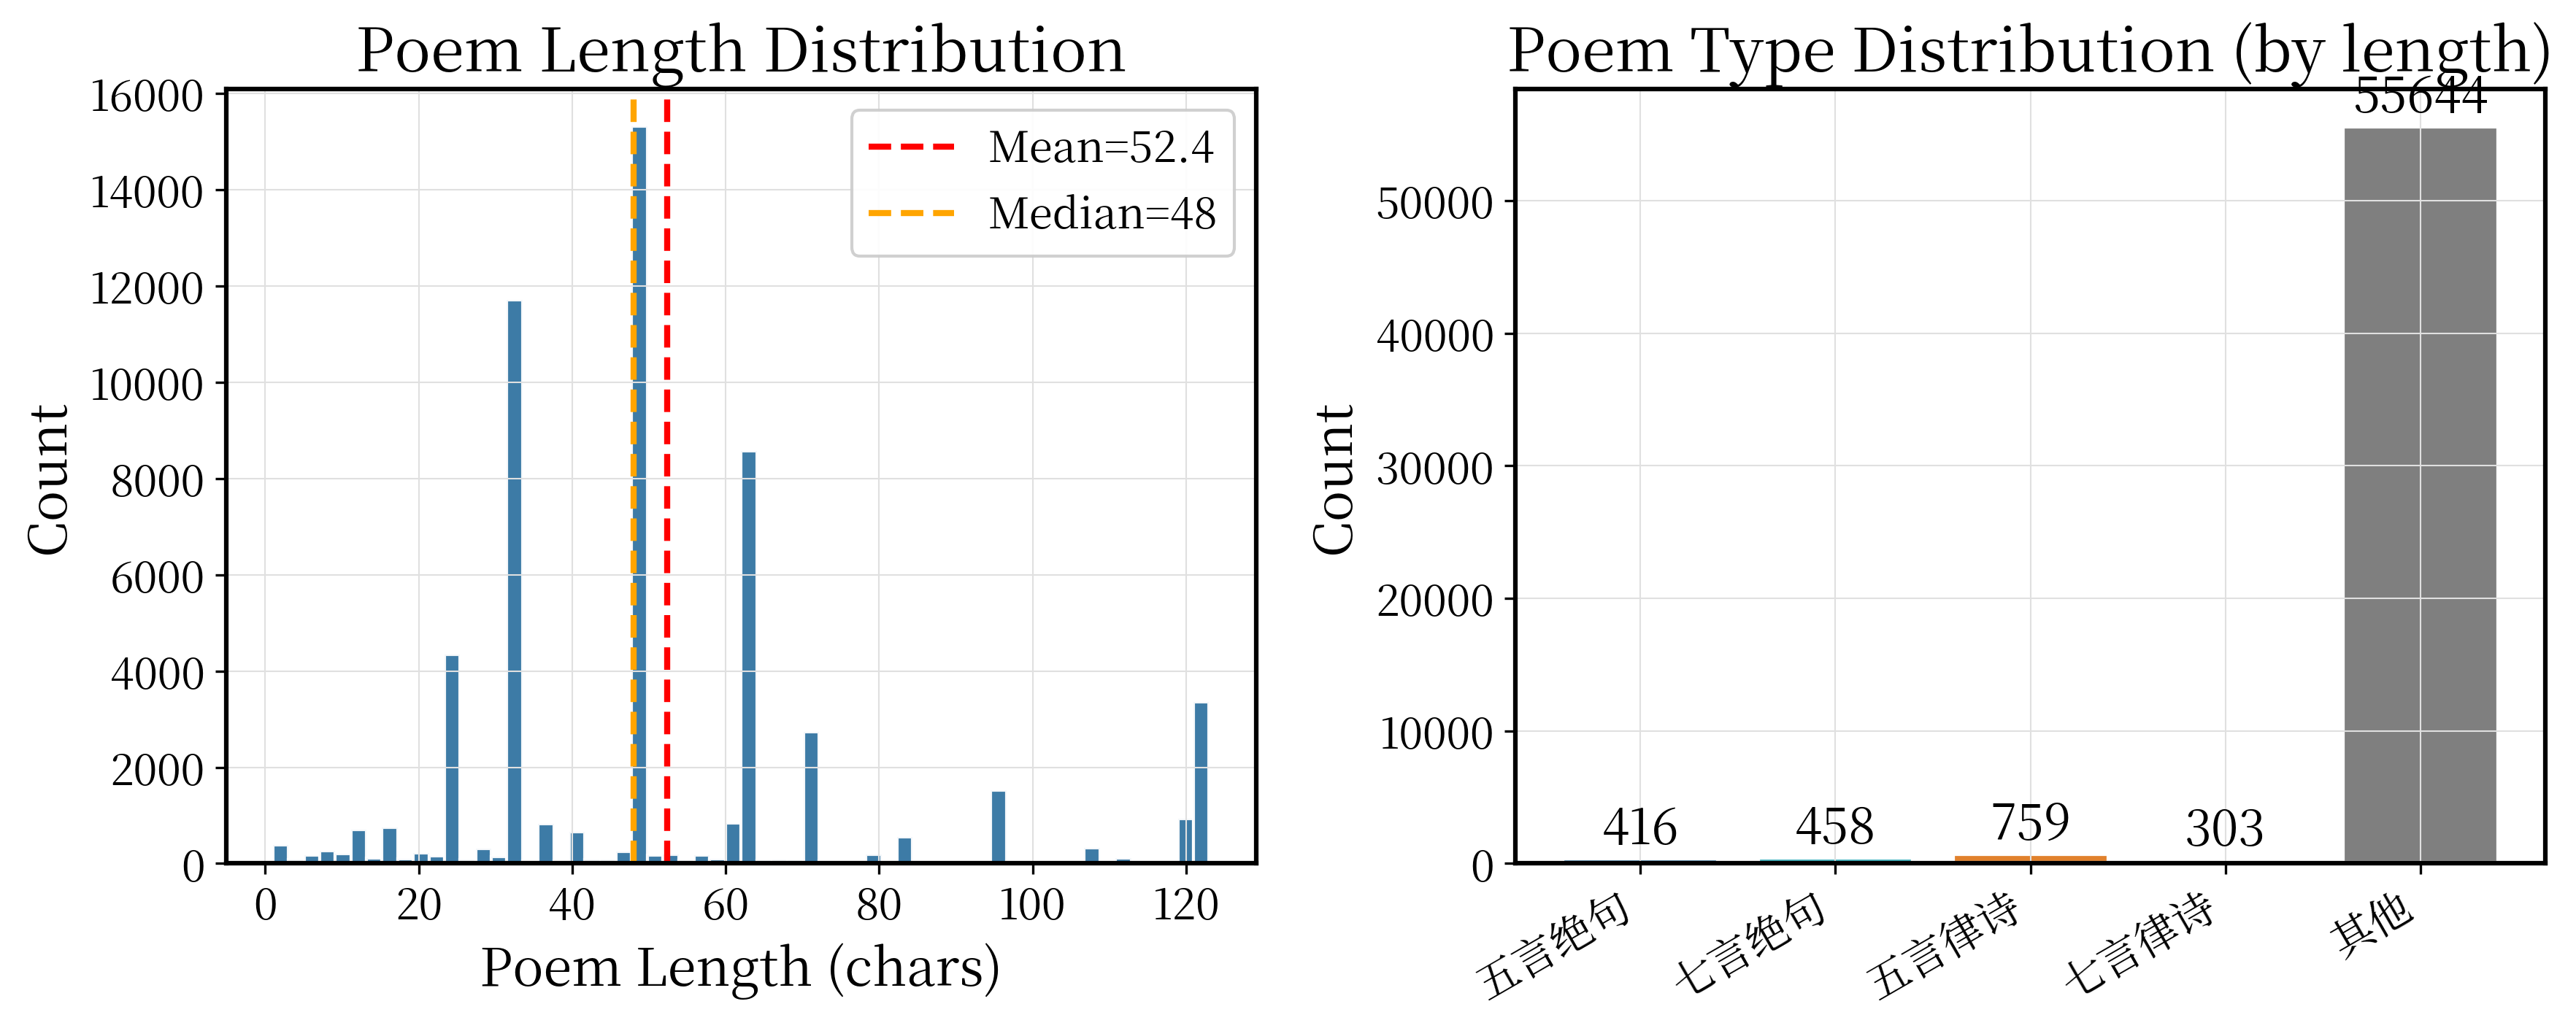
\includegraphics[width=\textwidth]{figs/fig01_dataset_length.png}
\caption{唐诗长度分布（左）与体裁分布估计（右）}
\label{fig:length}
\end{figure}

图\ref{fig:length}左图说明，诗歌长度分布呈现明显的\textbf{多峰特征}，在20字（五言绝句）、28字（七言绝句）、40字（五言律诗）、56字（七言律诗）处有显著的峰值。这说明唐诗并非一个均匀的连续序列数据集，而是由若干离散的格式类型组成的混合分布。右图的饼图显示五言诗占比最高，这意味着模型需要特别擅长建模5字一句的模式。

\subsection{句式结构分析}

\begin{figure}[H]
\centering
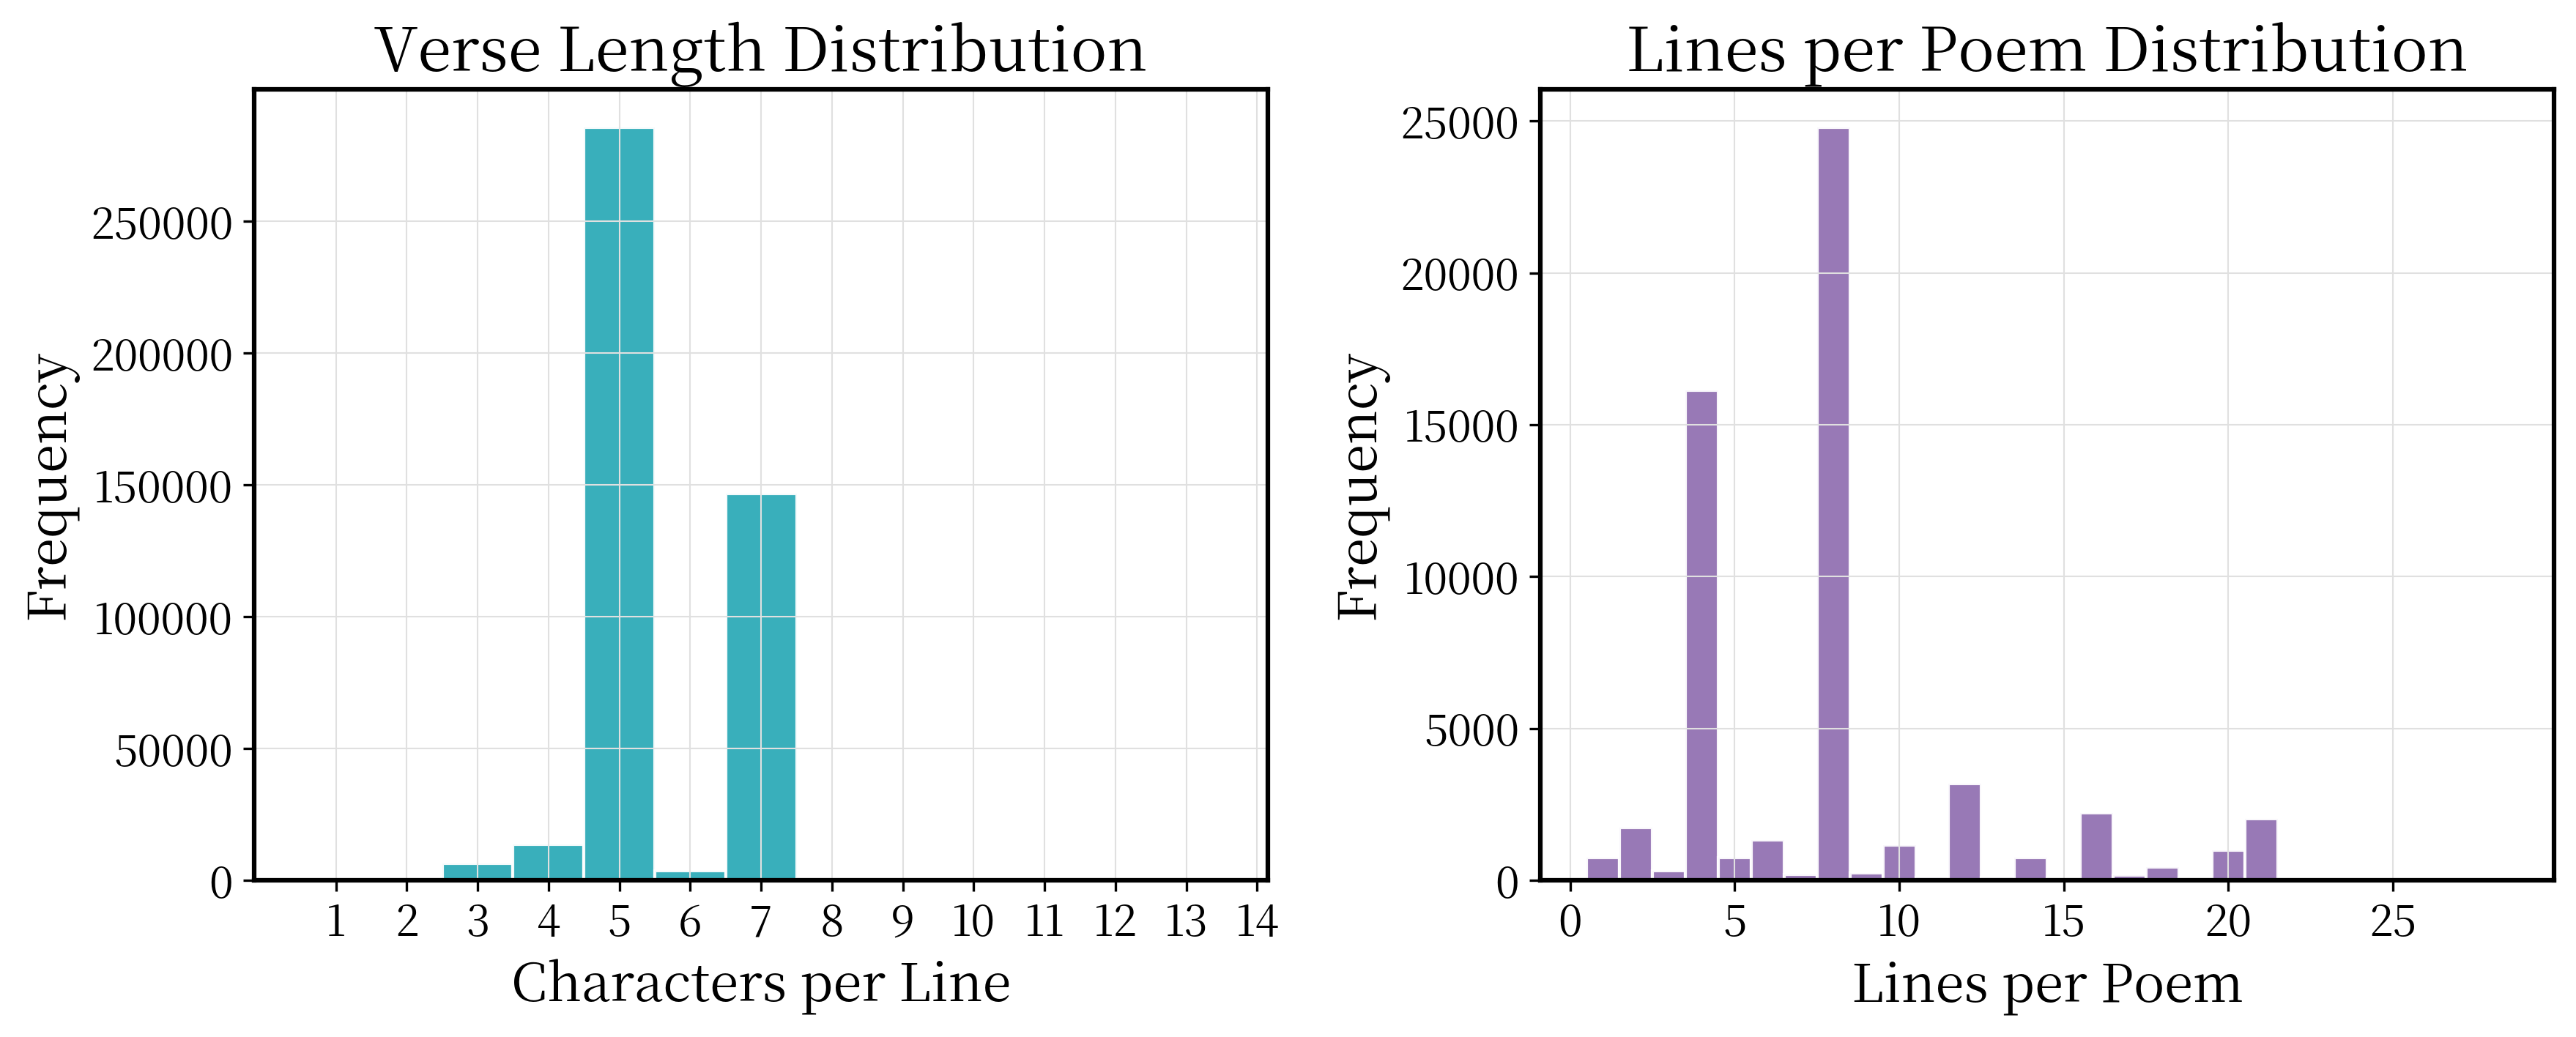
\includegraphics[width=\textwidth]{figs/fig10_structure.png}
\caption{诗句字数分布（左）与每首诗句数分布（右）}
\label{fig:structure}
\end{figure}

图\ref{fig:structure}进一步验证了，数据集中的诗的每一句的字数高度集中在5字和7字，几乎没有其他长度的句子。这意味着模型只需在两种句长模式间切换，降低了任务难度。句数分布则显示绝句和律诗为最常见形式。

% \subsection{字频分布与Zipf定律}

% \begin{figure}[H]
% \centering
% 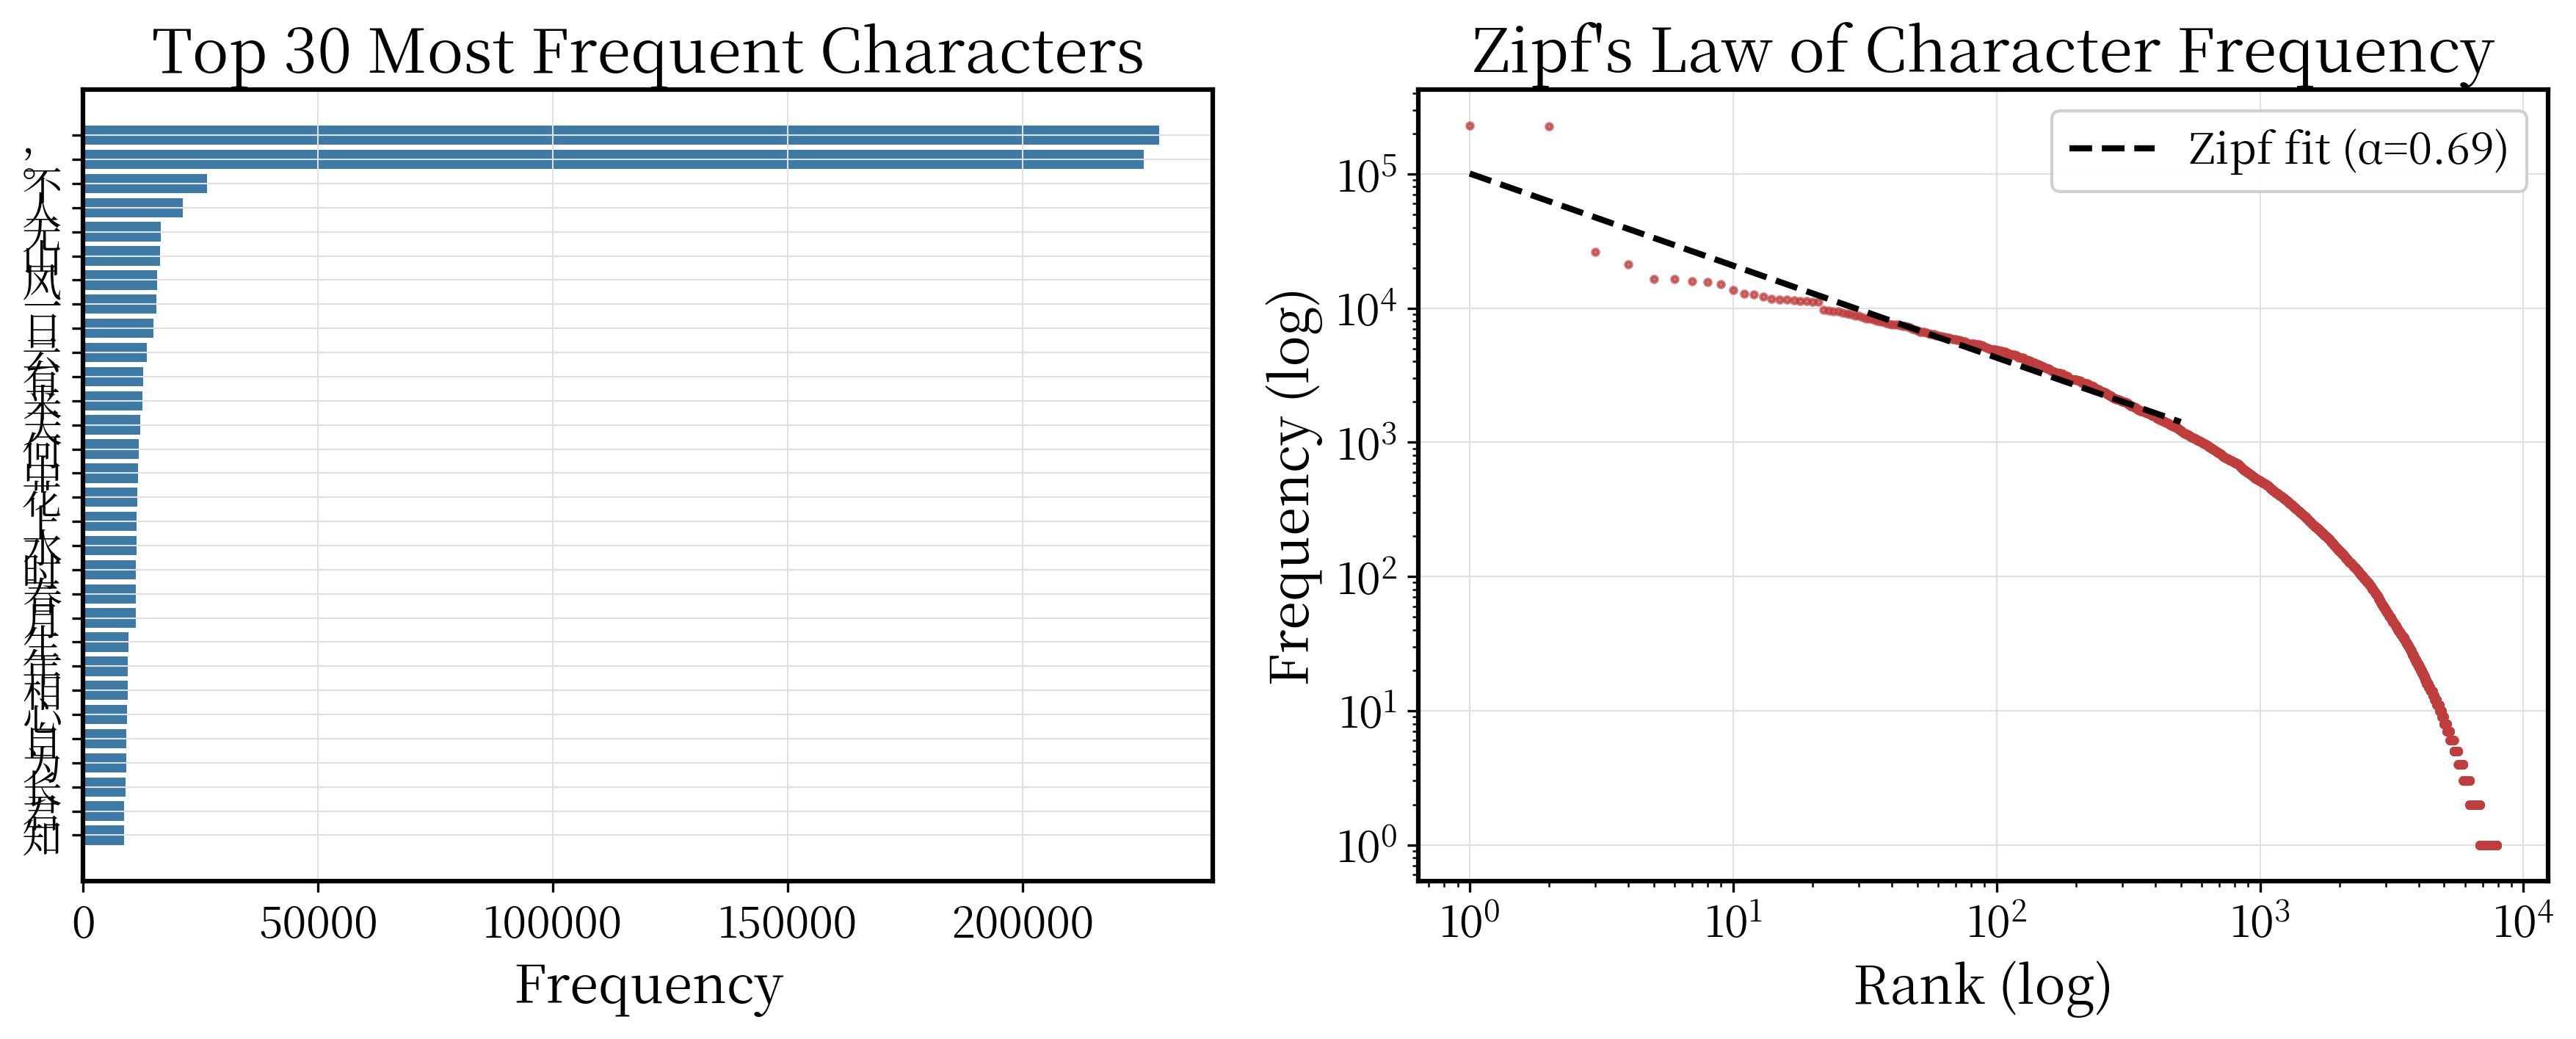
\includegraphics[width=\textwidth]{figs/fig02_char_frequency.png}
% \caption{高频字Top 30（左）与字频的Zipf分布验证（右）}
% \label{fig:charfreq}
% \end{figure}

% 图\ref{fig:charfreq}左图显示，最高频的字包括标点符号（逗号、句号）和常见虚词（"不""人""无""一"）。右图在双对数坐标下验证了字频服从\textbf{Zipf定律}，拟合指数$\alpha \approx 0.96$，接近经典值1。这意味着少量高频字占据了大部分出现次数，而大量低频字（生僻字）出现极少。

% \textbf{对训练的影响}：Zipf分布导致模型容易偏向生成高频字，而忽视低频但富有诗意的字。这也是为什么在生成时使用温度采样而非贪心解码——贪心解码会极端地偏向高频字。

\subsection{主题词频分析}

\begin{figure}[H]
\centering
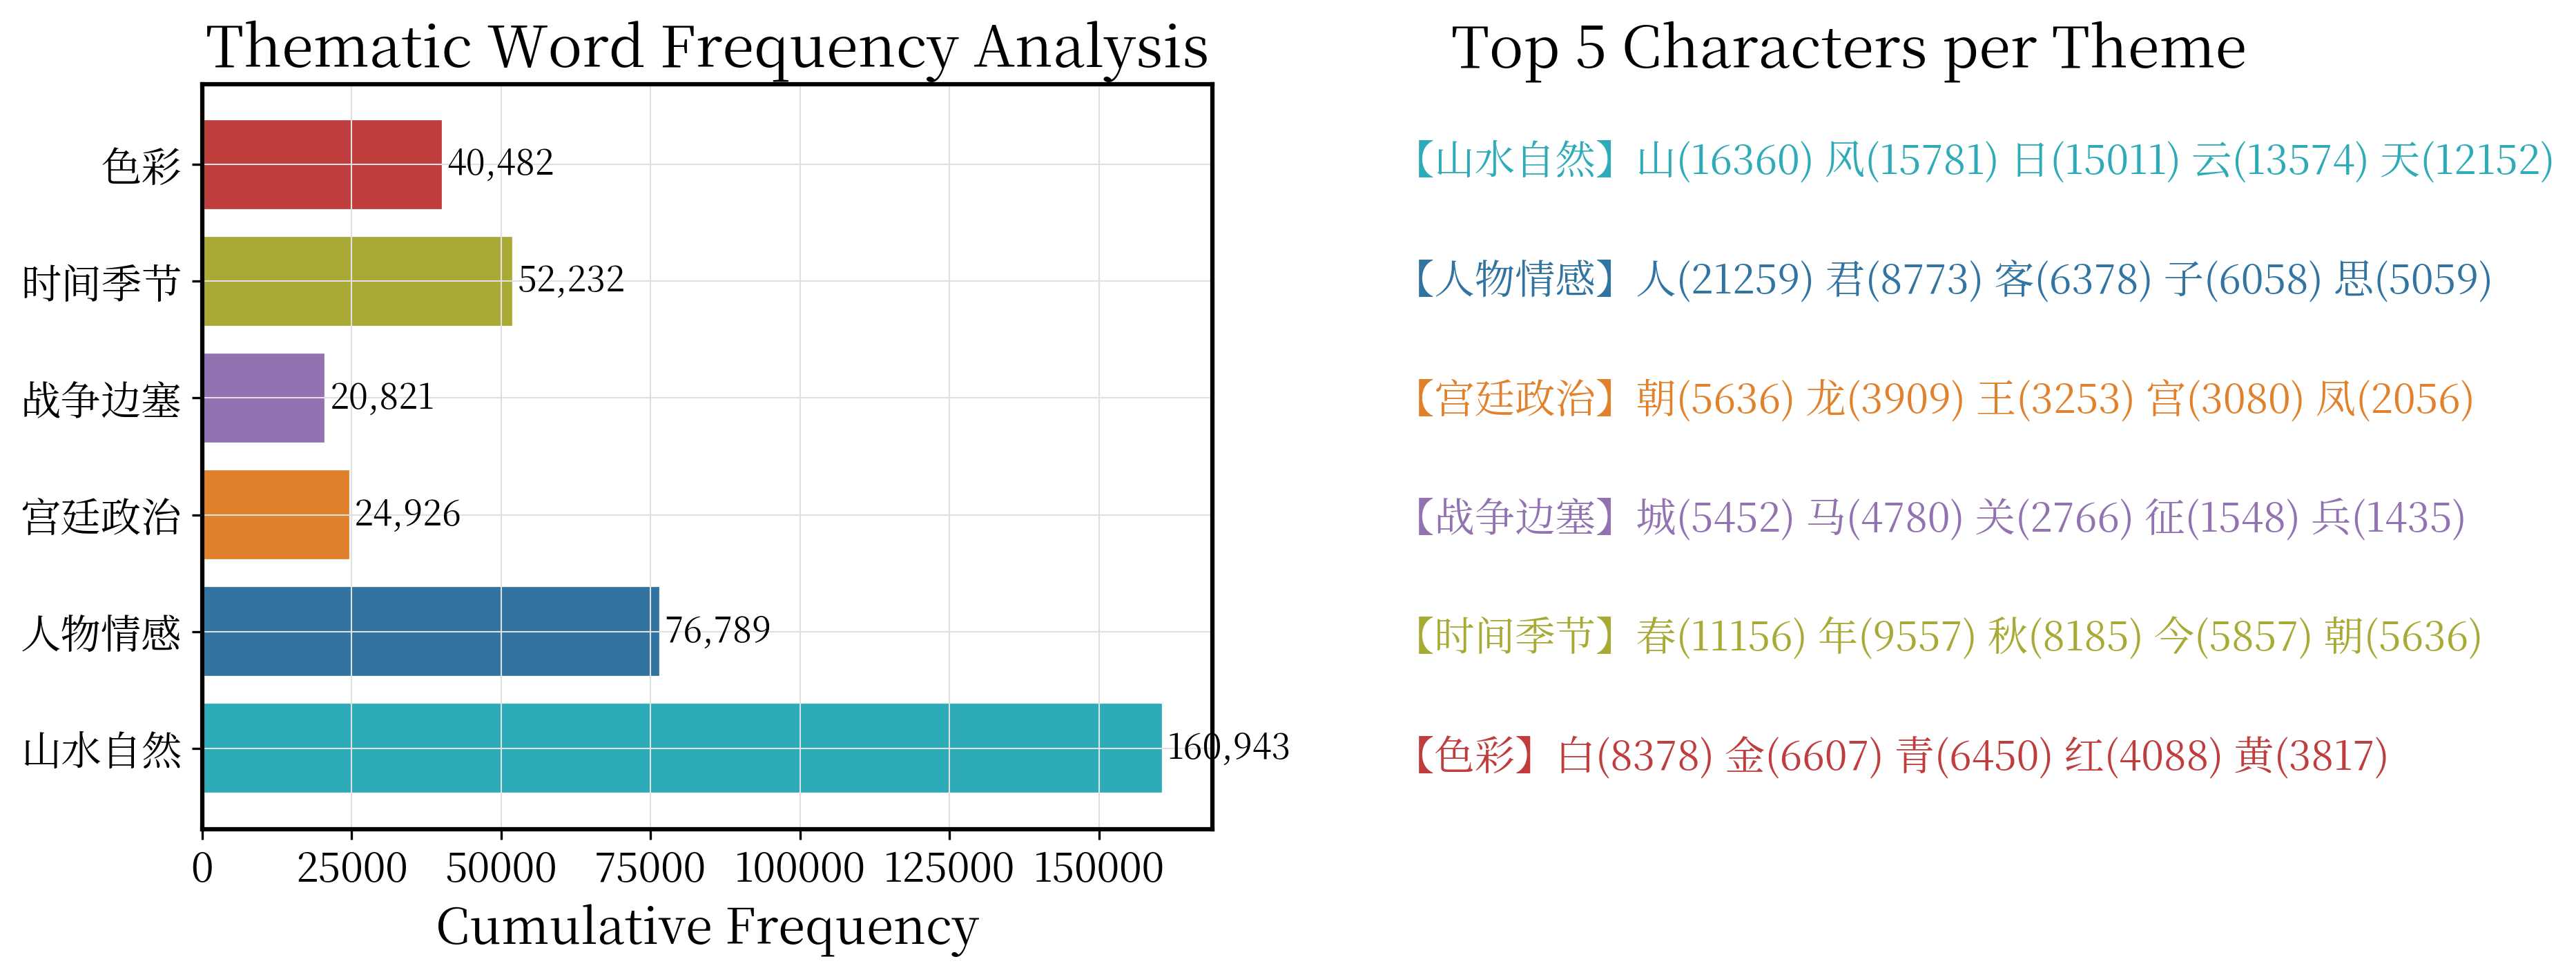
\includegraphics[width=\textwidth]{figs/fig11_themes.png}
\caption{唐诗主题词频分析}
\label{fig:themes}
\end{figure}

图\ref{fig:themes}将词汇按语义主题分组统计。"山水自然"和"人物情感"两大主题的总频次远超其他主题，这与唐诗以山水田园、离愁别绪为主流的文学特征完全吻合。"色彩"类字词中"白"和"青"频次最高，反映了唐诗偏好素雅清冷的色调美学。

\textbf{一个有趣的观察}："战争边塞"类虽然是唐诗四大流派之一，但其主题字频远低于"山水自然"。这可能是因为边塞诗的数量在全唐诗中占比较小，也可能是因为边塞诗使用了更多专有名词（地名、人名）而非本分析选取的通用主题词。

% ==============================================================
\section{模型设计与实现}
% ==============================================================

\subsection{三种模型架构}

为了进行充分的对比分析，本实验设计了三种不同复杂度的模型，核心思路是控制变量，分别考察网络深度、门控机制类型和模型容量对性能的影响。

\begin{table}[H]
\centering
\caption{三种模型架构对比}
\begin{tabular}{lcccccc}
\toprule
\textbf{模型} & \textbf{类型} & \textbf{嵌入维度} & \textbf{隐藏维度} & \textbf{层数} & \textbf{Dropout} & \textbf{参数量} \\
\midrule
Basic & LSTM & 128 & 256 & 1 & 0 & 3.59M \\
Deep  & LSTM & 256 & 512 & 3 & 0.3 & 12.16M \\
GRU   & GRU  & 256 & 512 & 2 & 0.2 & 9.14M \\
\bottomrule
\end{tabular}
\end{table}

\textbf{Basic模型}：作为基线，使用最简单的单层LSTM，与实验指导书的示例一致。它的参数量最小，训练最快，但容量有限。

\textbf{Deep模型}：通过增加到3层、扩大维度来提升容量，同时引入Dropout防止过拟合，低层捕获字面的n-gram模式，高层捕获更抽象的语义和韵律模式。

\textbf{GRU模型}：使用2层GRU替代LSTM，既然GRU参数更少，那么在相同隐藏维度下它应该更不容易过拟合；同时2层的深度介于Basic（1层）和Deep（3层）之间，提供了一个中间参考点。

\begin{figure}[H]
\centering
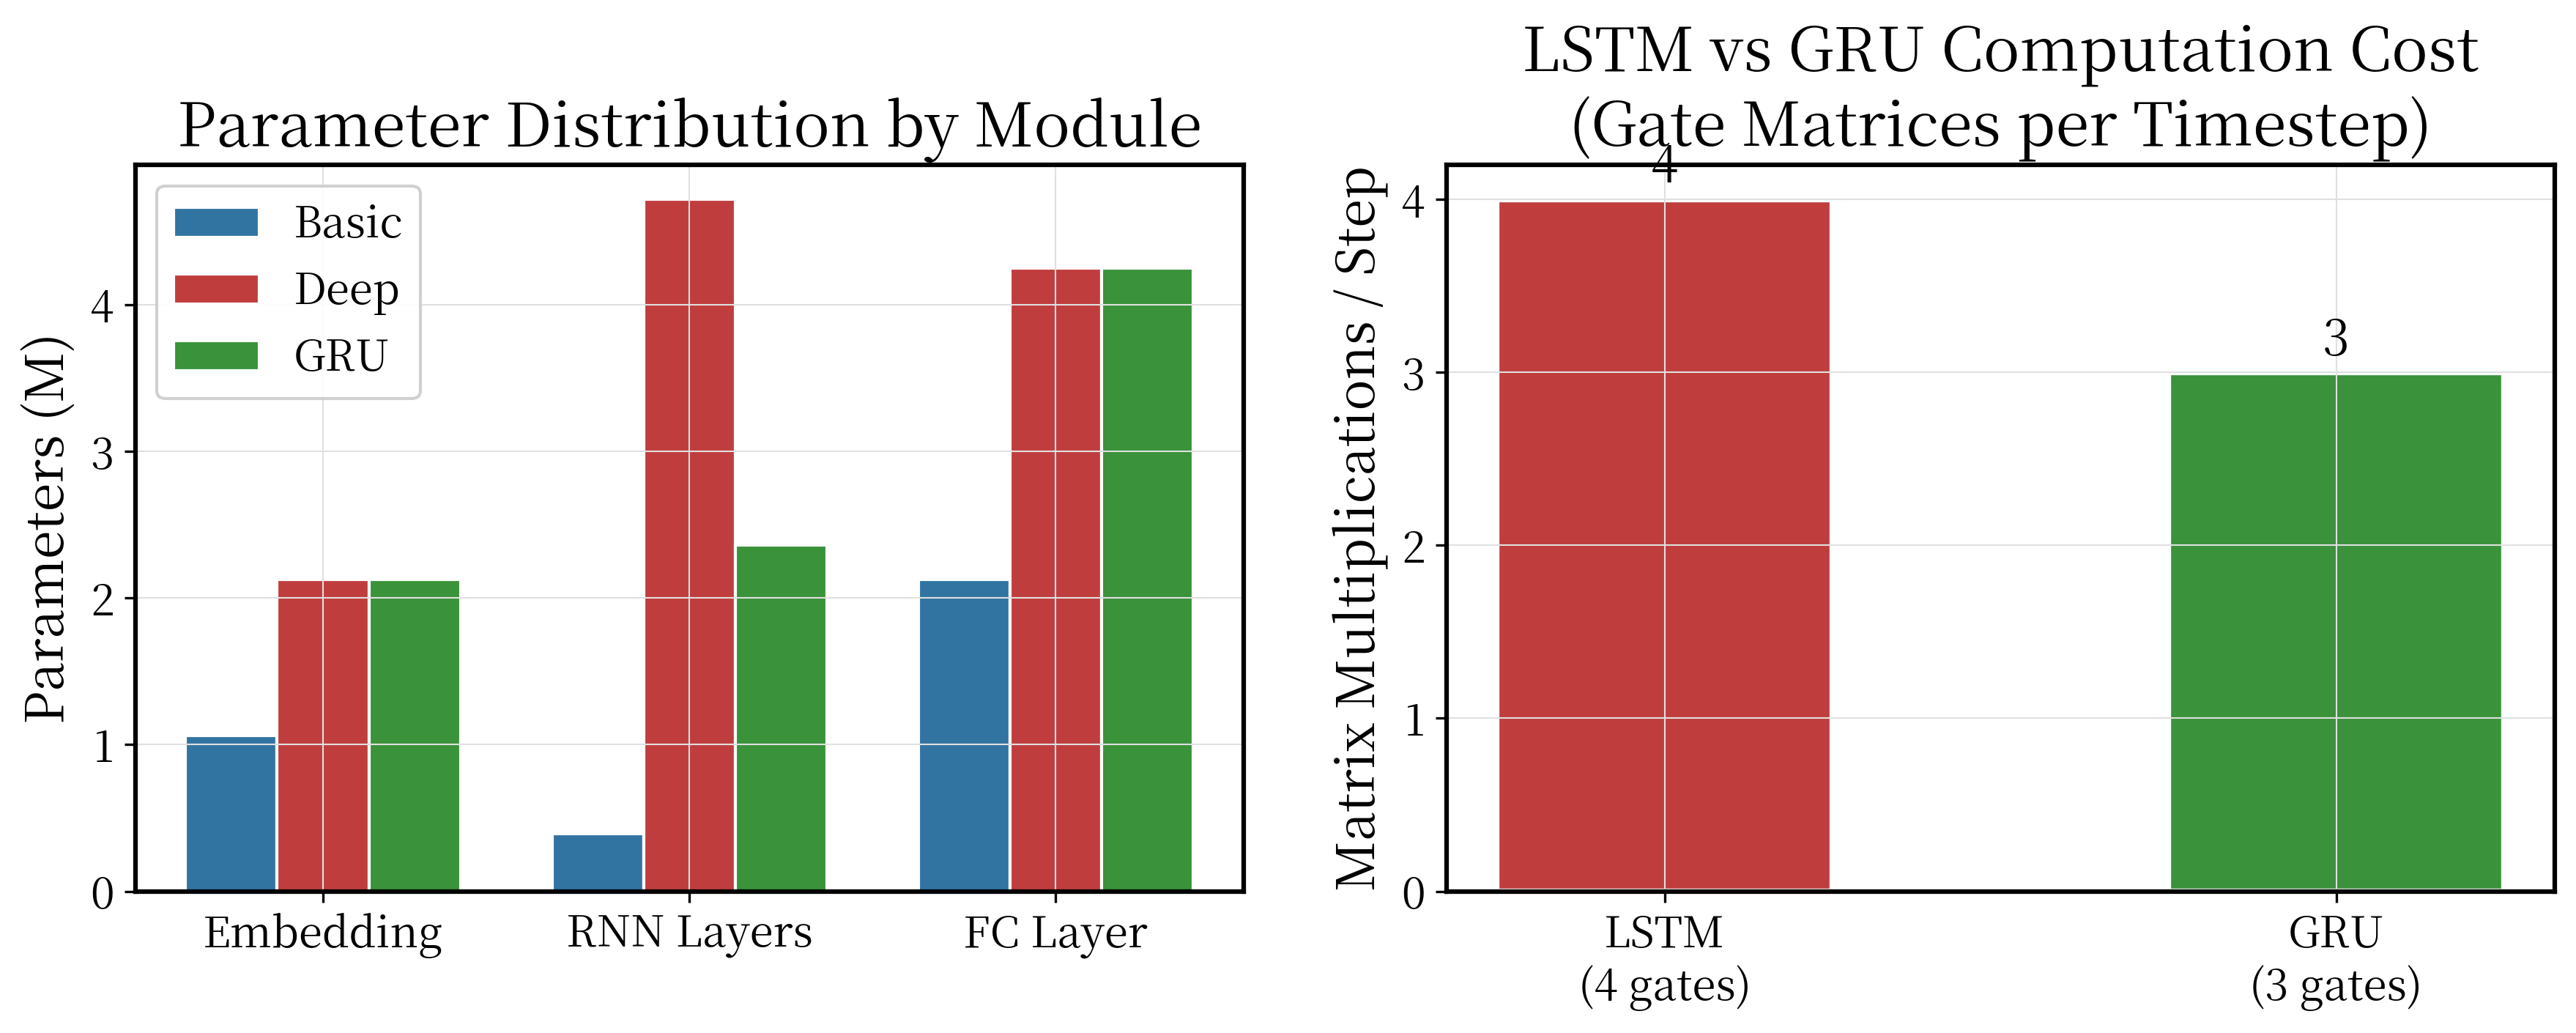
\includegraphics[width=\textwidth]{figs/fig14_architecture.png}
\caption{各模块参数量分布（左）与LSTM/GRU门控计算量对比（右）}
\label{fig:arch}
\end{figure}

图\ref{fig:arch}对三种模型的参数量进行了分析，\textbf{Embedding层和全连接层的参数量占比极大}，尤其是Basic模型中RNN层本身的参数只占一小部分。这是因为词汇表大小(8293)远大于隐藏维度，导致输入/输出投影矩阵成为参数瓶颈。这意味着简单地增加RNN层数并不能线性提升模型容量。

\subsection{训练配置}

\begin{table}[H]
\centering
\caption{训练配置参数}
\begin{tabular}{ccc}
\toprule
参数 & 配置 & 设计理由 \\
\midrule
优化器 & Adam & 自适应学习率，适合RNN训练 \\
初始学习率 & $1 \times 10^{-3}$ & RNN训练的常用初始值 \\
学习率调度 & StepLR (×0.5, 每10ep) & 分阶段衰减，观察衰减效果 \\
损失函数 & CrossEntropyLoss & 字符级语言模型的标准选择 \\
梯度裁剪 & max\_norm=5.0 & 防止LSTM/GRU中的梯度爆炸 \\
批大小 & 64 & GPU内存与训练速度的平衡 \\
训练轮次 & 30 epochs & 观察到收敛后停止 \\
\bottomrule
\end{tabular}
\end{table}

% \textbf{关于梯度裁剪的思考}：虽然LSTM/GRU通过门控机制缓解了梯度消失，但梯度爆炸仍然可能发生——尤其是在多层网络中，梯度通过多层的残差路径累积。设置max\_norm=5.0是一个保守的选择，确保训练稳定性。

\subsection{生成策略}

\subsubsection{温度采样}

给定模型输出的logits $z_i$，通过温度参数$\tau$调节采样分布：
\begin{equation}
    P(w_i) = \frac{\exp(z_i / \tau)}{\sum_j \exp(z_j / \tau)}
\end{equation}

$\tau < 1$使分布更尖锐（更保守），$\tau > 1$使分布更平坦（更冒险）。本实验使用$\tau = 0.8$。

\subsubsection{藏头诗生成}

藏头诗在每句开头强制使用指定字符，其余位置自回归生成。检测到标点后，下一个字由藏头序列指定而非模型生成，但仍将该字输入模型以维护隐状态的连贯性。

% ==============================================================
\section{实验结果与分析}
% ==============================================================

\subsection{训练过程分析}

\subsubsection{损失与困惑度曲线}
图\ref{fig:loss_ppl}展示了三种模型在30个epoch内的训练轨迹。整体来看，GRU从第3个epoch开始loss低于Deep LSTM，并在后续训练中保持领先，说明参数量增加并不必然带来性能提升，模型结构与训练数据的适配性同样重要。Basic LSTM后期曲线趋于平坦，基本停止改善，而GRU和Deep LSTM仍有轻微下降趋势，表明二者可能仍具备进一步优化空间。困惑度方面，GRU最终达到PPL=5.01，相当于每个位置平均在约5个候选字中选择，相较于8293的词汇量，模型预测已较为确定。

\begin{figure}[H]
\centering
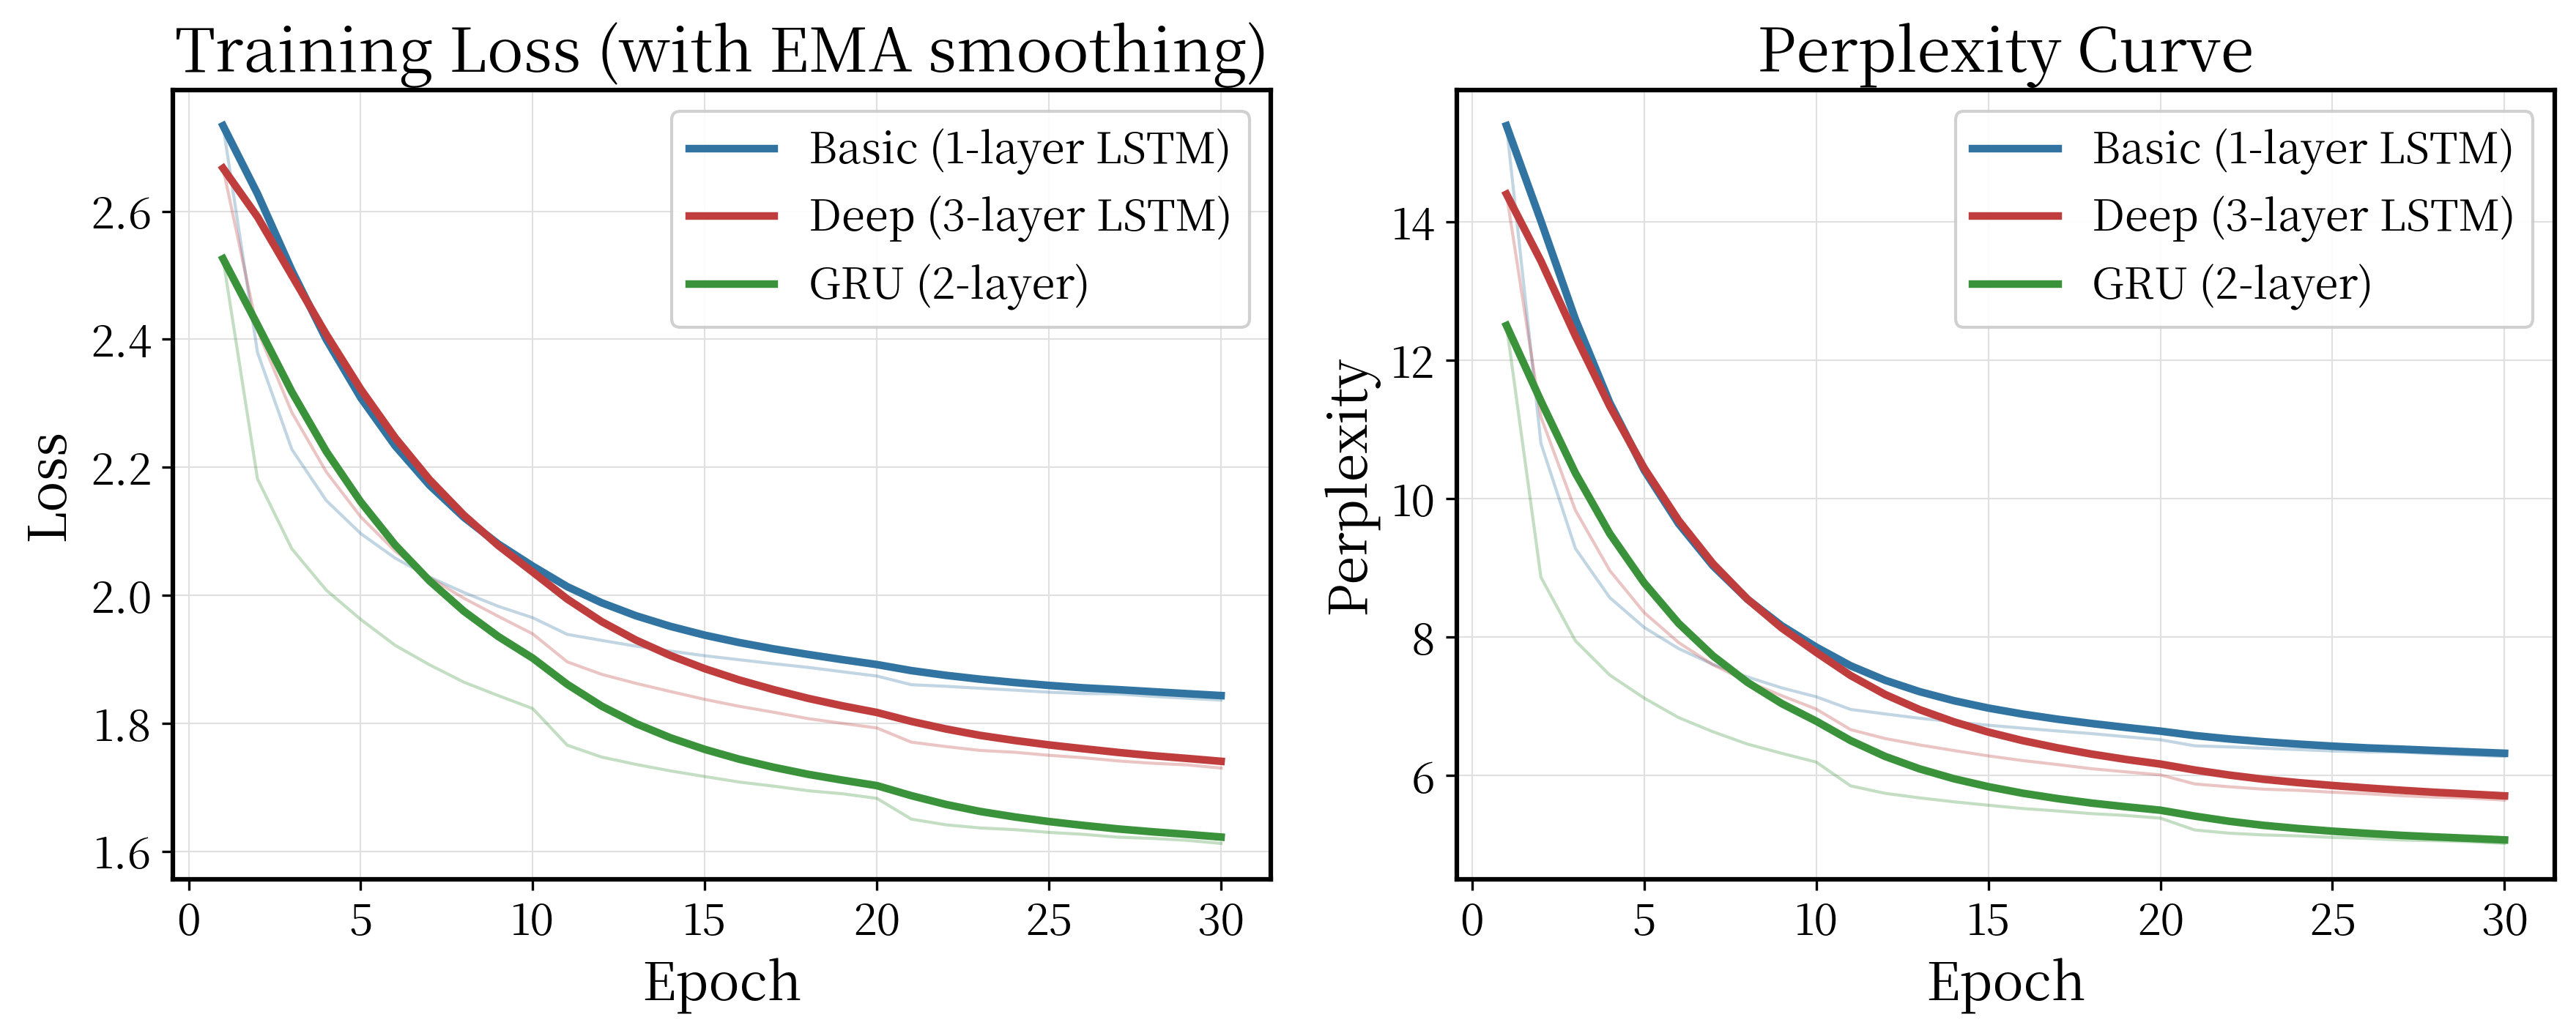
\includegraphics[width=\textwidth]{figs/fig03_loss_ppl.png}
\caption{训练损失曲线（左）与困惑度变化（右），含EMA平滑}
\label{fig:loss_ppl}
\end{figure}

% 图\ref{fig:loss_ppl}展示了三种模型30个epoch的训练轨迹。几个关键观察：

% \begin{enumerate}[leftmargin=*]
%     \item \textbf{GRU全程领先}：从第3个epoch开始，GRU的loss就低于Deep LSTM，尽管后者参数量多33\%。这个结果在一定程度上出乎意料——通常我们认为更多参数=更强的模型。后文将详细分析原因。
%     \item \textbf{曲线形态差异}：Basic LSTM的曲线在后期非常平坦，几乎停止改善；而GRU和Deep LSTM仍有微弱的下降趋势，暗示它们可能在更多epoch后进一步提升。
%     \item \textbf{PPL的绝对值}：最优模型GRU达到PPL=5.01，意味着每个位置模型平均在5个候选字中选择。考虑到8293的词汇量，这是$5/8293=0.06\%$的搜索空间，模型已经非常"确定"下一个字应该是什么。
% \end{enumerate}

\begin{table}[H]
\centering
\caption{模型最终性能对比}
\label{tab:final}
\begin{tabular}{lcccc}
\toprule
\textbf{模型} & \textbf{最终Loss} & \textbf{最终PPL} & \textbf{参数量} & \textbf{训练时间/epoch} \\
\midrule
Basic LSTM & 1.836 & 6.27 & 3.59M & $\sim$19.5s \\
Deep LSTM  & 1.730 & 5.64 & 12.16M & $\sim$62.0s \\
GRU        & \textbf{1.612} & \textbf{5.01} & 9.14M & $\sim$47.6s \\
\bottomrule
\end{tabular}
\end{table}

% \subsubsection{训练三阶段分析}

% \begin{figure}[H]
% \centering
% 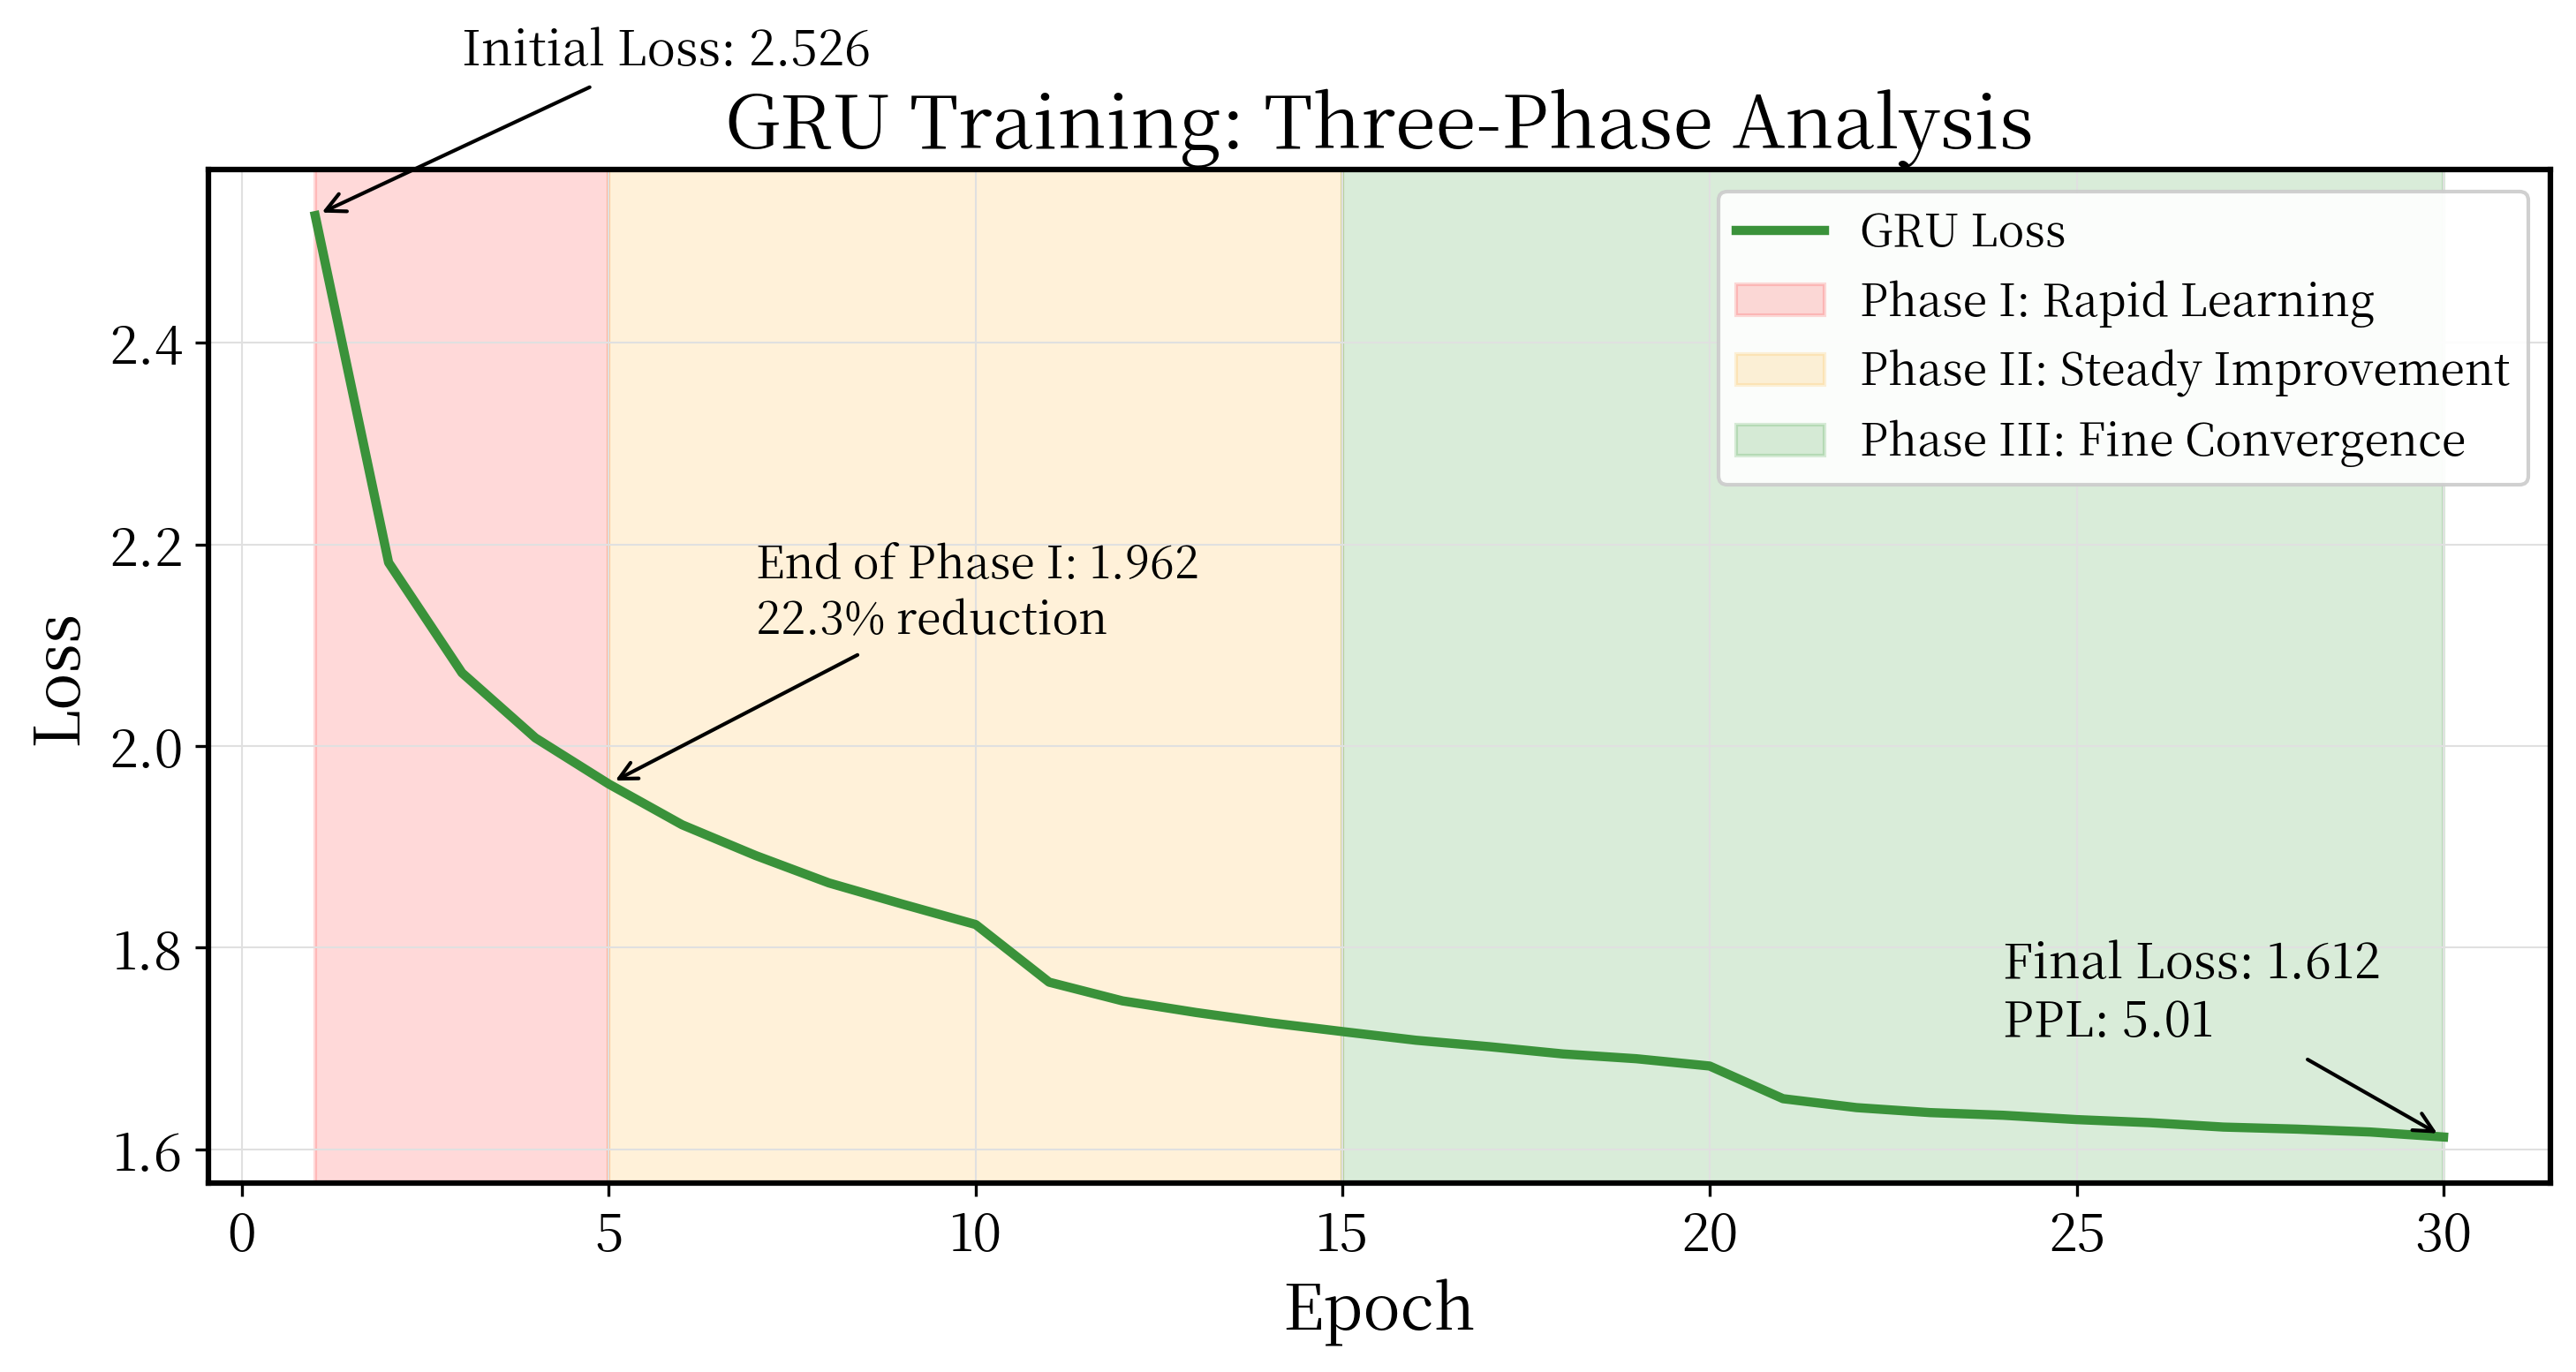
\includegraphics[width=\textwidth]{figs/fig13_phases.png}
% \caption{GRU模型训练过程的三阶段划分}
% \label{fig:phases}
% \end{figure}

% 以表现最好的GRU模型为例，图\ref{fig:phases}将30个epoch的训练过程划分为三个阶段：

% \textbf{Phase I（快速学习期，ep 1--5）}：Loss从2.526急剧下降至1.962，改善了22.3\%。这一阶段模型快速学习了最基本的语言规律——哪些字经常出现、标点符号的位置模式、五言/七言的节奏等。从信息论角度看，模型在此阶段消除了最多的"不确定性"。

% \textbf{Phase II（稳定改善期，ep 5--15）}：Loss以稳定但递减的速率从1.962下降至1.717。模型在此阶段学习更精细的语言模式——字与字之间的搭配关系、对仗工整性、意象的连贯性等。

% \textbf{Phase III（精细收敛期，ep 15--30）}：Loss仅从1.717下降至1.612，每epoch改善不足0.5\%。模型已接近其容量极限，进一步的改善可能需要增加模型容量或数据量。

\subsubsection{收敛速度与学习率衰减的效果}

\begin{figure}[H]
\centering
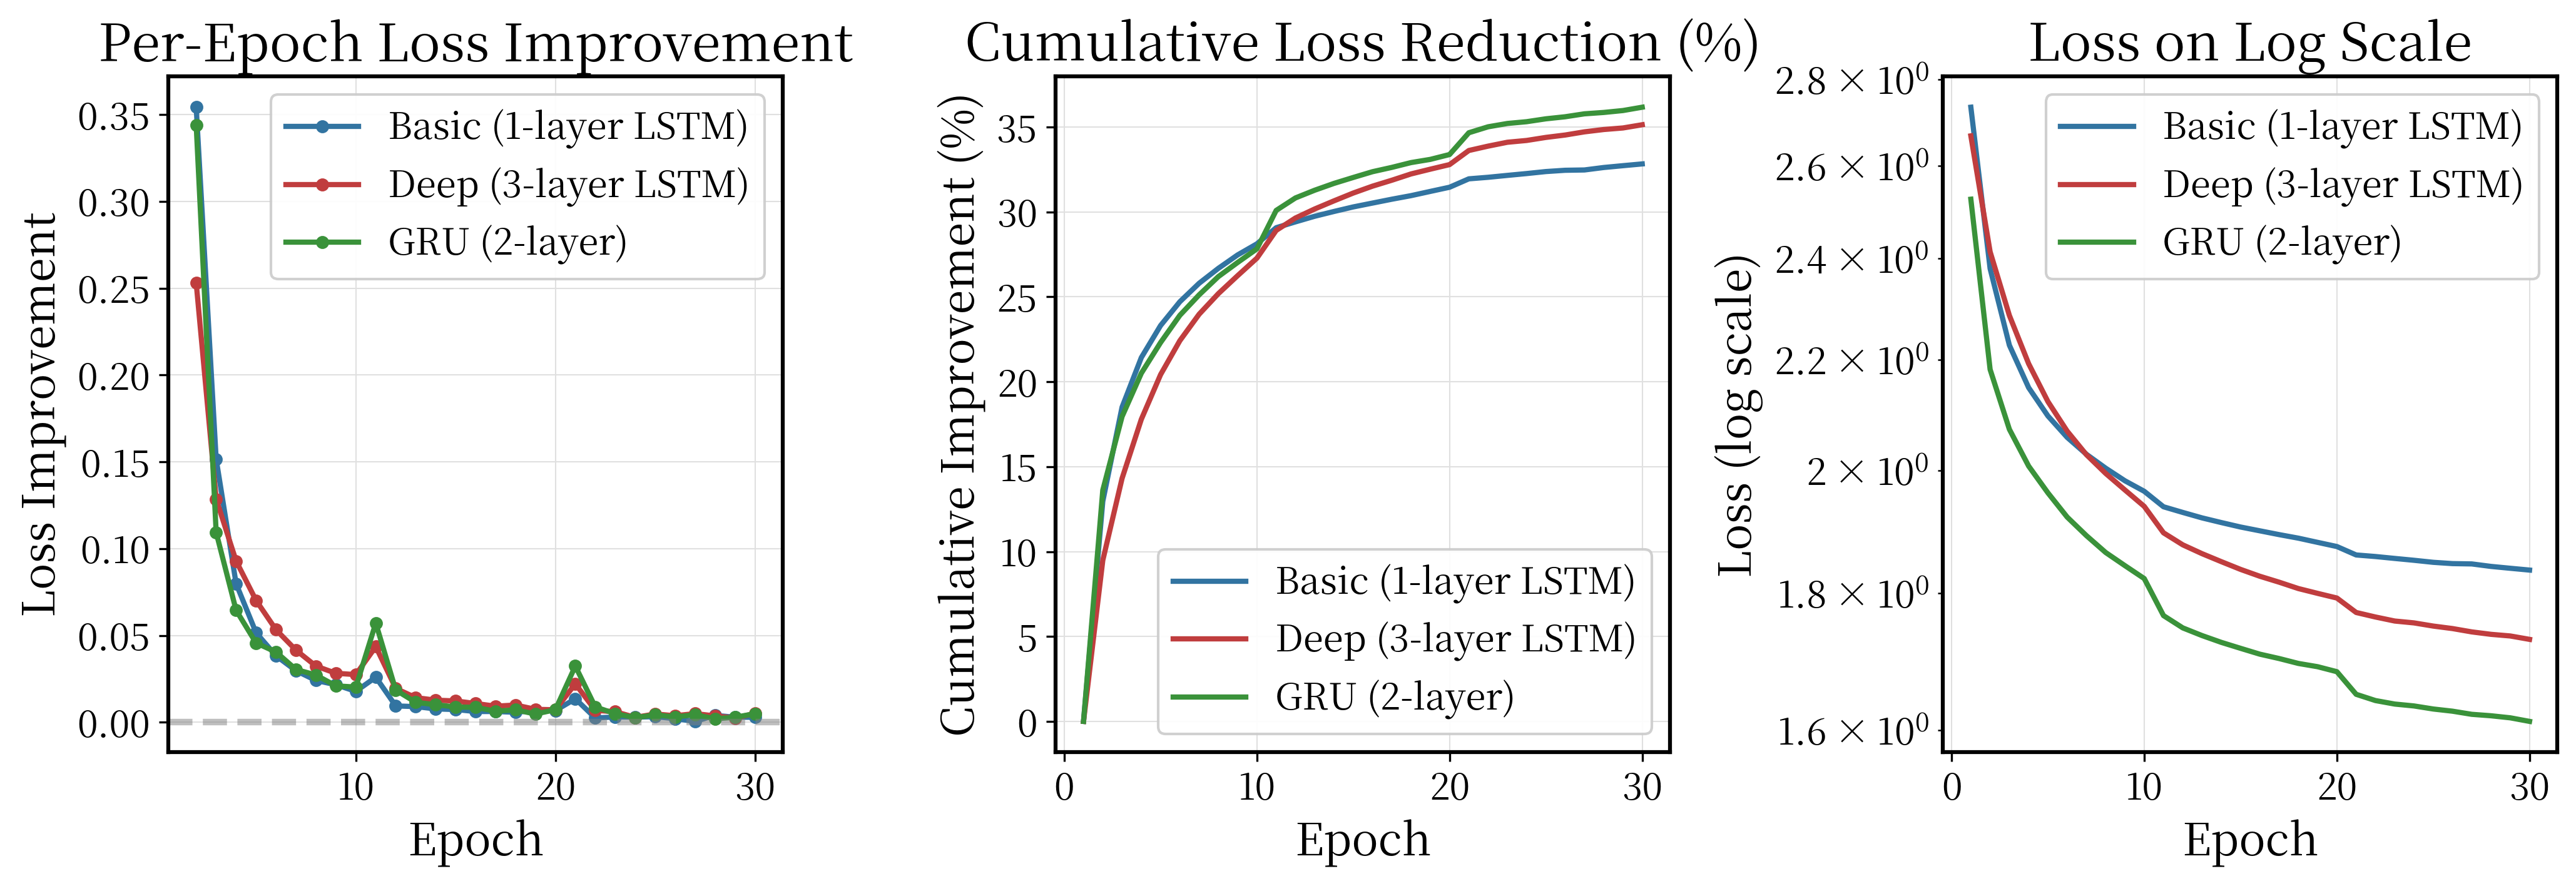
\includegraphics[width=\textwidth]{figs/fig04_convergence.png}
\caption{收敛动态分析：(左) 每epoch改善量 (中) 累计改善率 (右)}
\label{fig:convergence}
\end{figure}

图\ref{fig:convergence}展示了三种模型的收敛动态。可以看出，随着训练推进，每个epoch带来的loss改善逐渐减小，说明模型整体趋于收敛。但在epoch 10和epoch 20附近，改善量出现短暂上升，表明学习率衰减对训练过程产生了一定促进作用。

\begin{figure}[H]
\centering
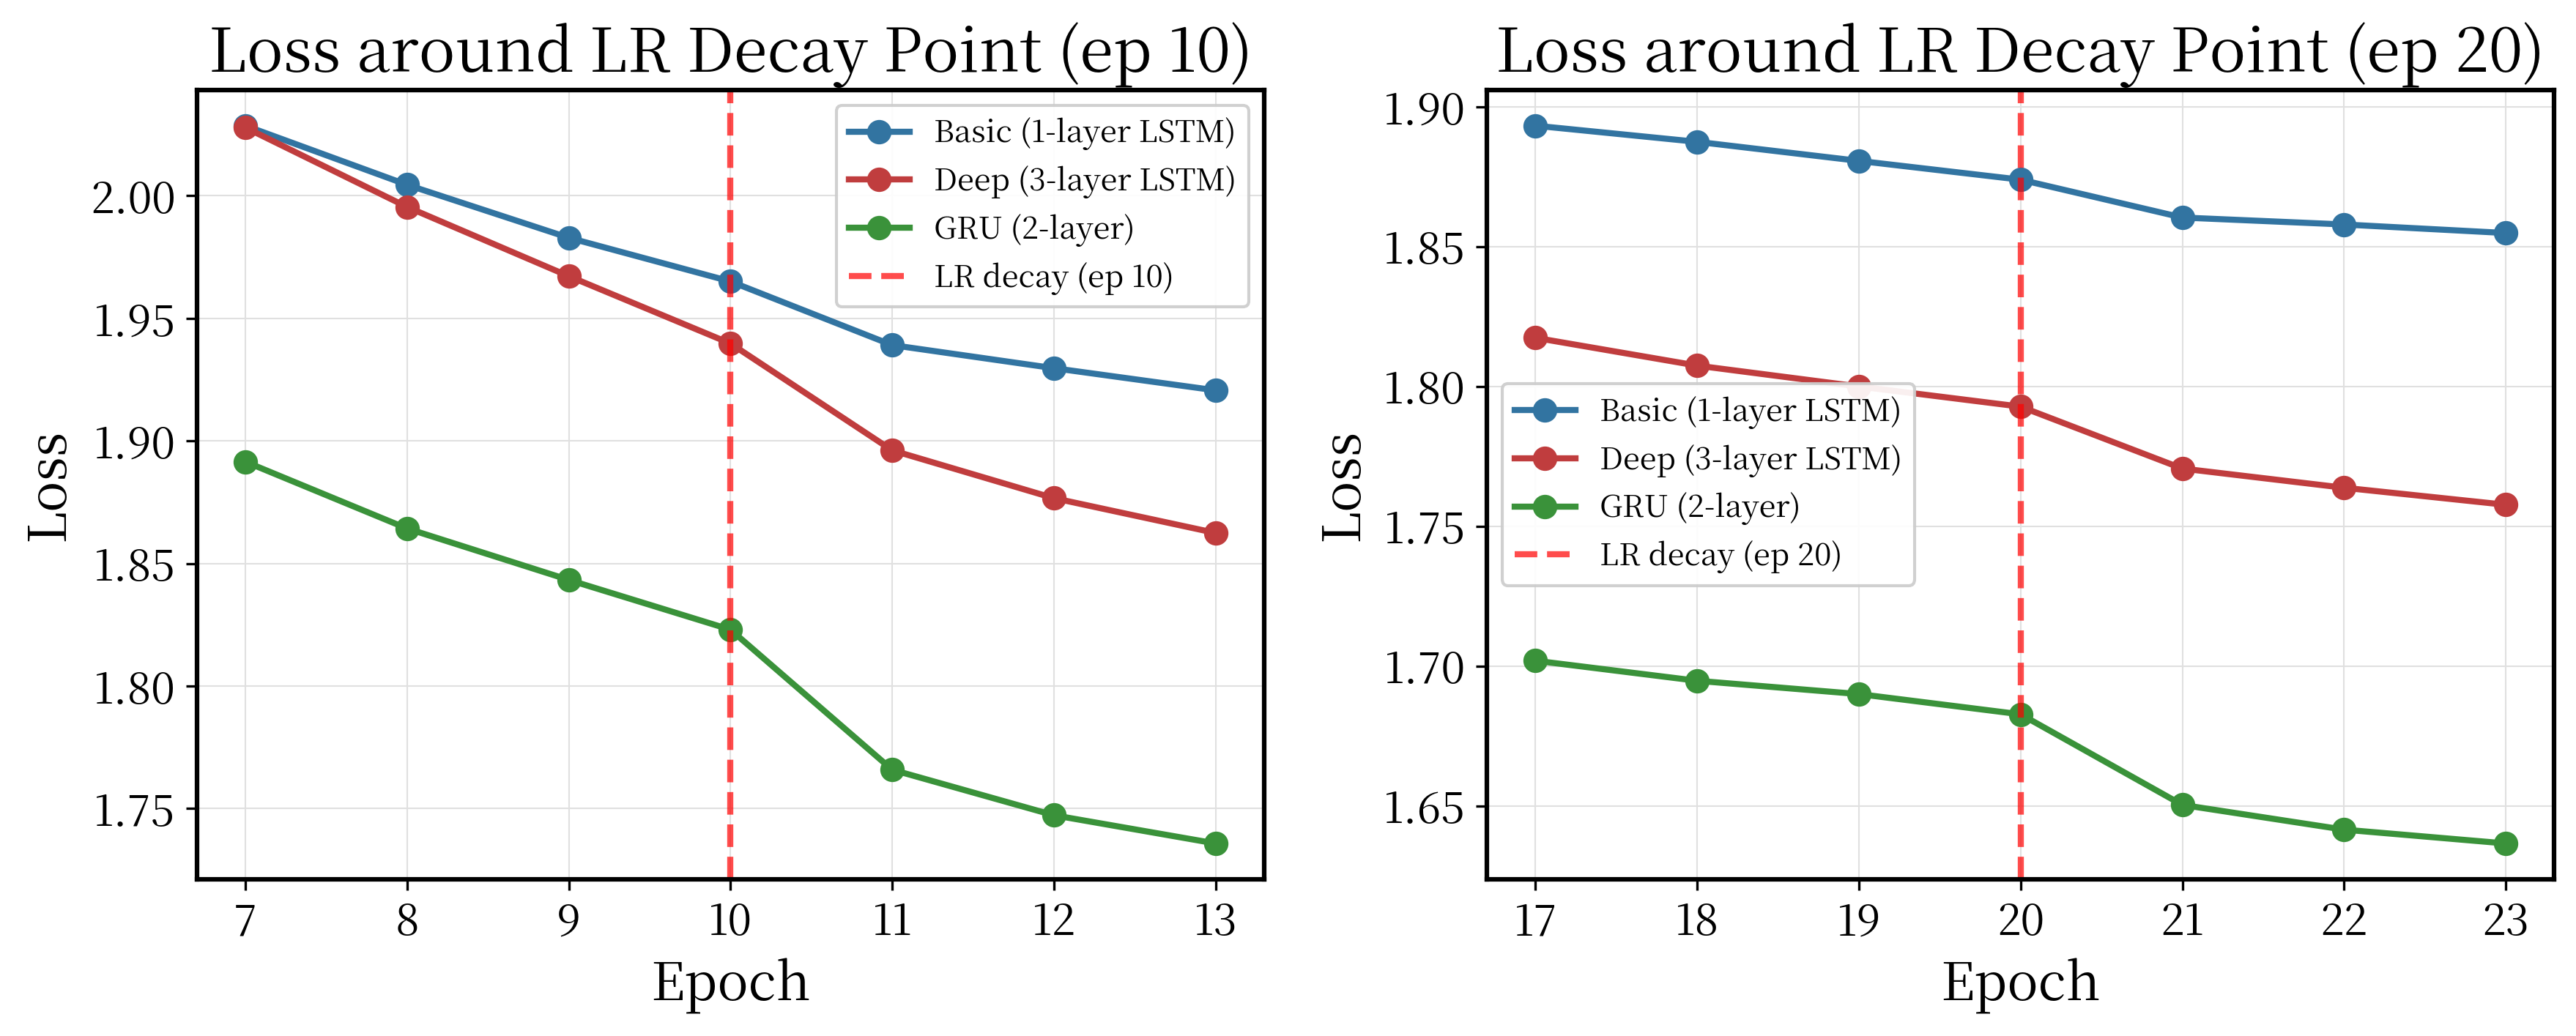
\includegraphics[width=\textwidth]{figs/fig12_lr_decay_impact.png}
\caption{学习率衰减点附近的Loss变化细节}
\label{fig:lr_impact}
\end{figure}

图\ref{fig:lr_impact}进一步展示了学习率衰减前后的loss变化。在epoch 10处，学习率由$10^{-3}$降至$5\times10^{-4}$后，三种模型的loss下降速度均出现短暂提升，说明较小学习率有助于模型在后期更稳定地逼近最优解。相比之下，epoch 20处的第二次衰减效果较弱，说明此时模型已经接近收敛，继续降低学习率带来的提升有限。

\subsection{模型综合对比}

% \subsubsection{性能-效率图}

\begin{figure}[H]
\centering
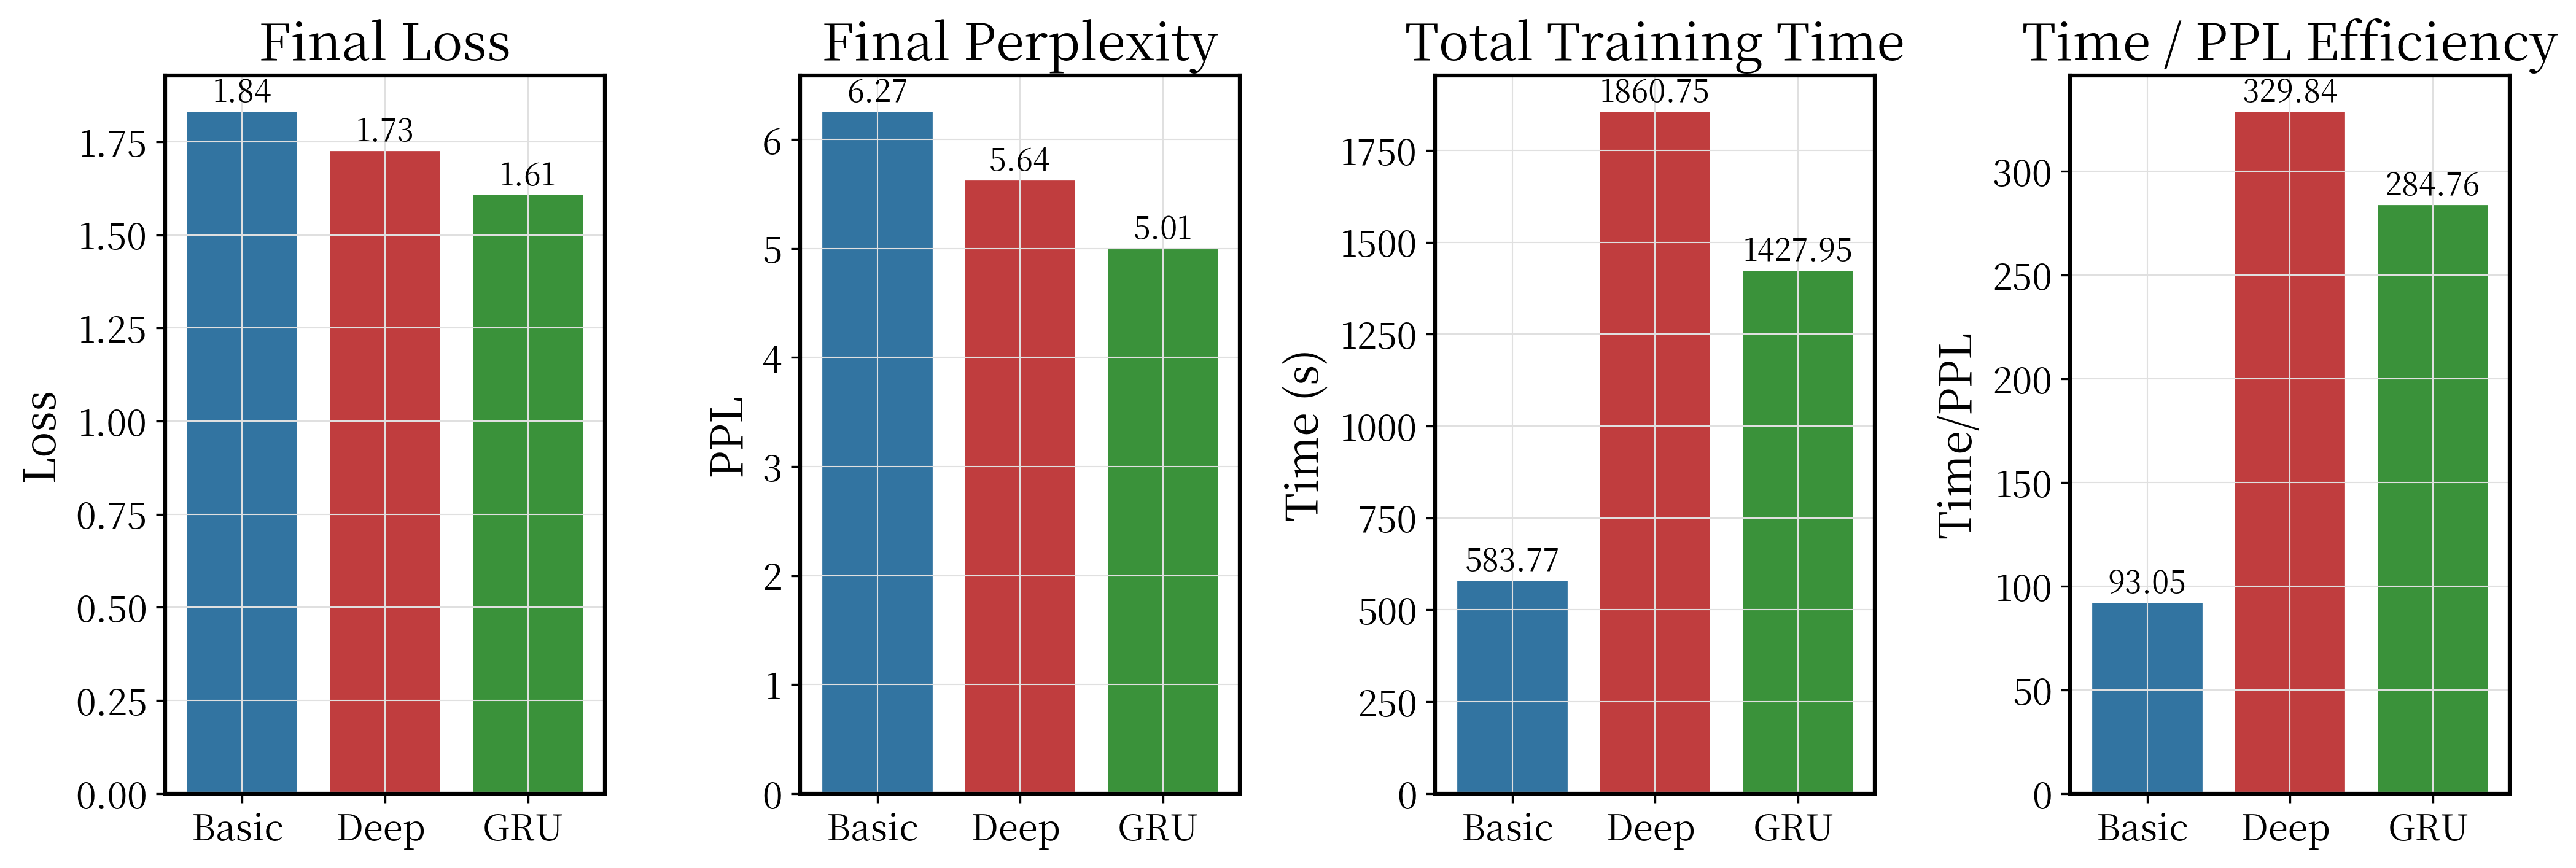
\includegraphics[width=\textwidth]{figs/fig06_summary.png}
\caption{三种模型最终指标综合对比}
\label{fig:summary}
\end{figure}

图\ref{fig:summary}对三种模型的最终性能与训练效率进行了综合比较。可以看出，GRU在PPL、loss以及训练效率等指标上均表现较优，说明其不仅具有更好的预测效果，也能以较低的训练成本获得更稳定的性能提升。相比之下，Deep LSTM虽然参数量更大，但并未带来更优结果，表明在本任务中，模型结构的适配性比单纯增加模型规模更为重要。

% \subsubsection{参数效率分析}

% \begin{figure}[H]
% \centering
% 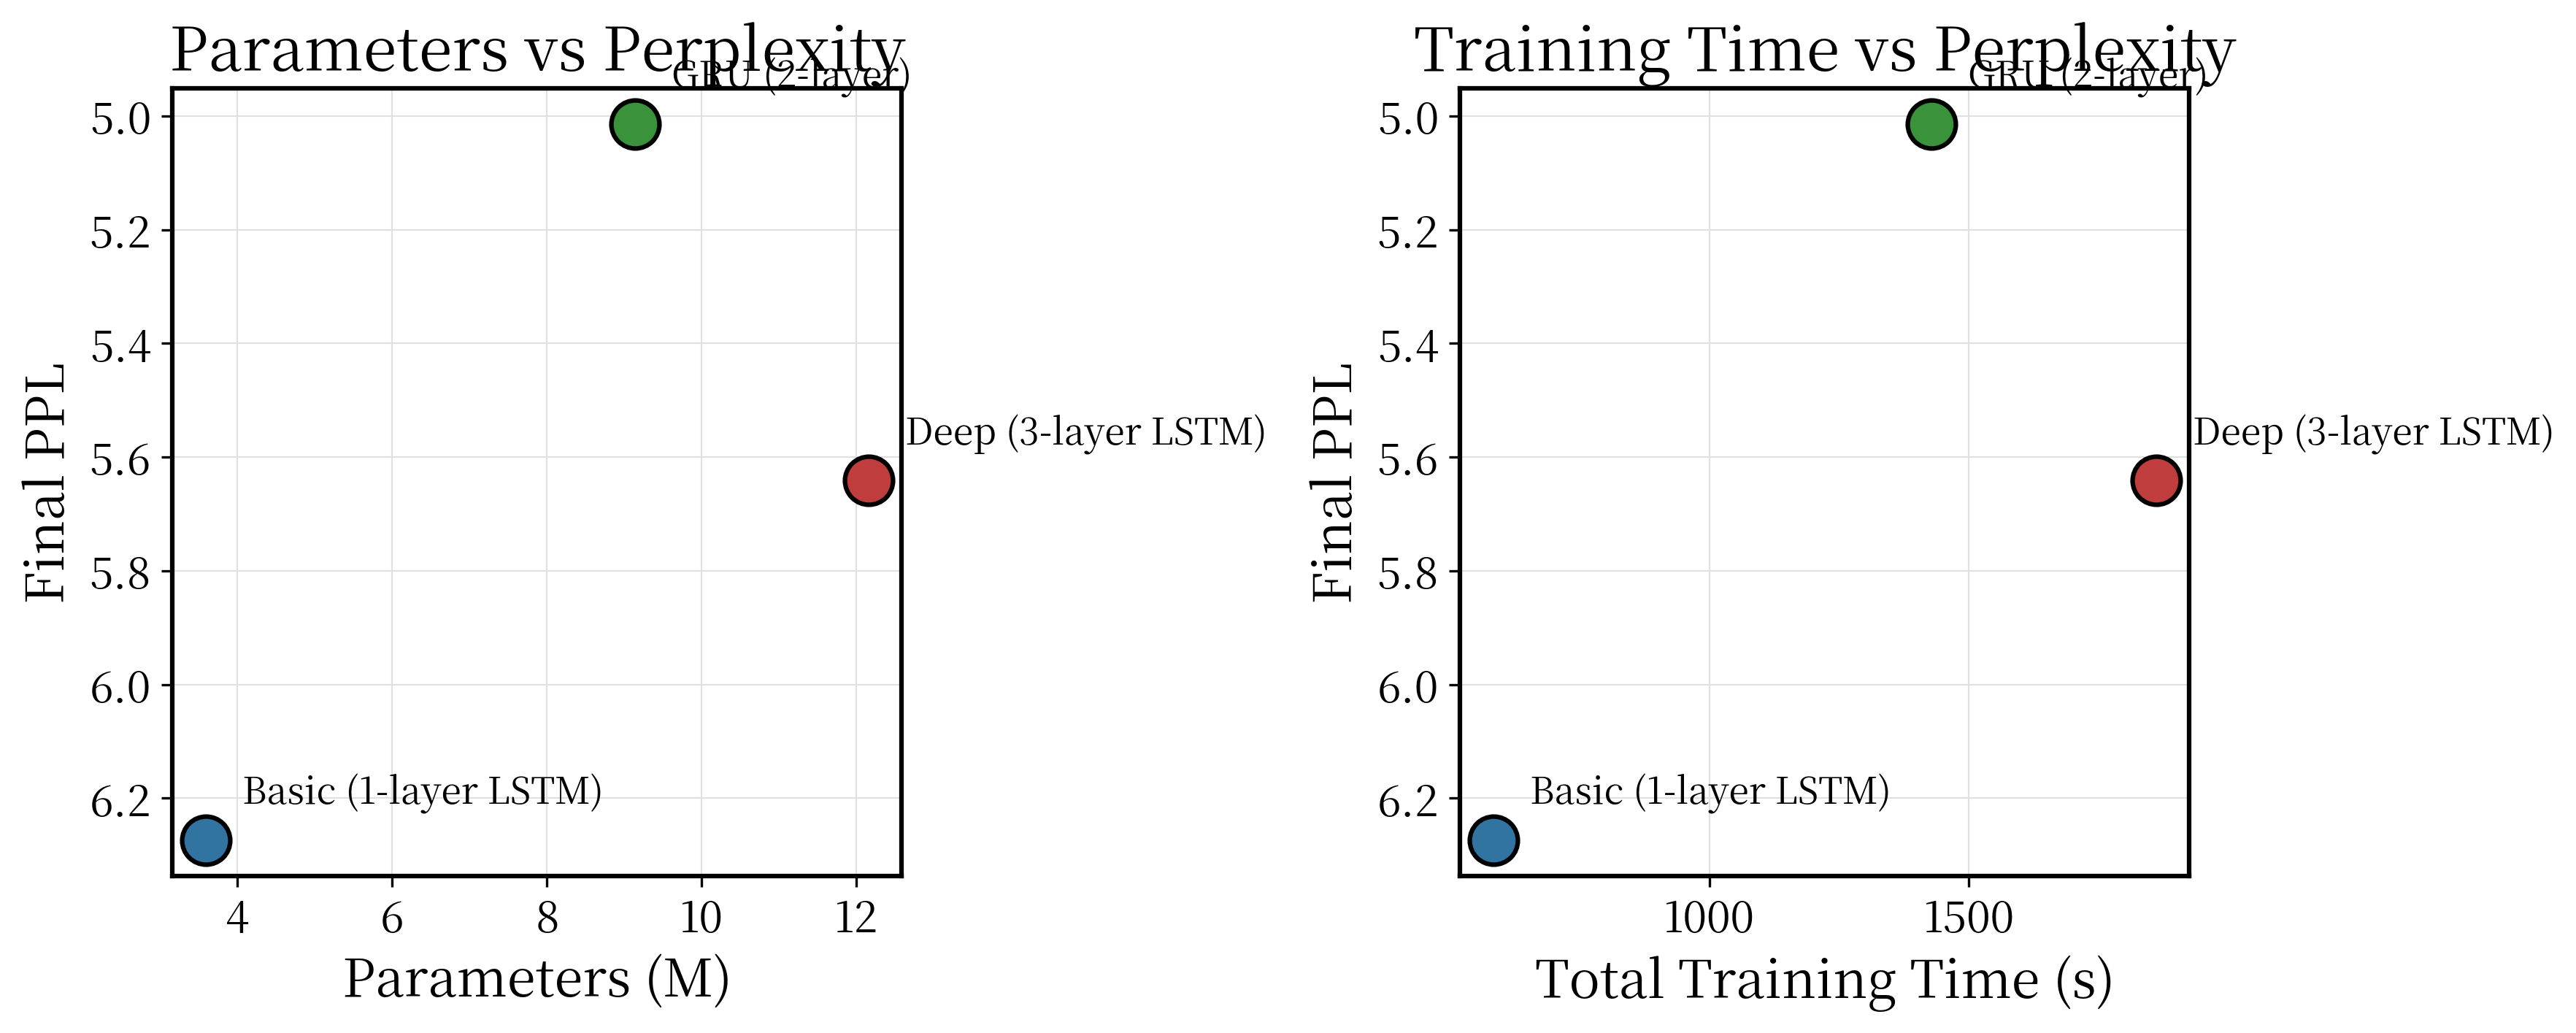
\includegraphics[width=\textwidth]{figs/fig07_efficiency.png}
% \caption{参数量(左)和训练时间(右)与困惑度的关系}
% \label{fig:efficiency}
% \end{figure}

% 图\ref{fig:efficiency}清晰地展示了一个\textbf{反直觉的现象}：参数量最多的Deep LSTM（12.16M）并非性能最好的模型。GRU以少27\%的参数（9.14M vs 12.16M）达到了更低的困惑度（5.01 vs 5.64）。

% \textbf{我对这一现象的解释}有三个层面：
% \begin{enumerate}[leftmargin=*]
%     \item \textbf{过拟合风险}：57,580首唐诗的数据规模对12M参数的模型而言偏小。Deep LSTM的0.3 Dropout虽然缓解了过拟合，但也"浪费"了一部分模型容量。
%     \item \textbf{优化难度}：3层LSTM的梯度传播路径更长、更复杂。尽管LSTM的门控机制缓解了梯度消失，但深层网络的loss surface更加崎岖，Adam优化器可能难以在30个epoch内找到好的局部最优。
%     \item \textbf{GRU的结构优势}：GRU的更新门$z_t$直接在"保留"和"更新"之间做线性插值（$(1-z_t) \cdot h_{t-1} + z_t \cdot \tilde{h}_t$），这是一种隐式的残差连接，使梯度流动更加顺畅。而LSTM的信息必须经过$f_t$、$i_t$、$o_t$三道门的"筛选"，每道门都可能成为梯度的瓶颈。
% \end{enumerate}

% \subsubsection{PPL达标速度对比}

% \begin{figure}[H]
% \centering
% 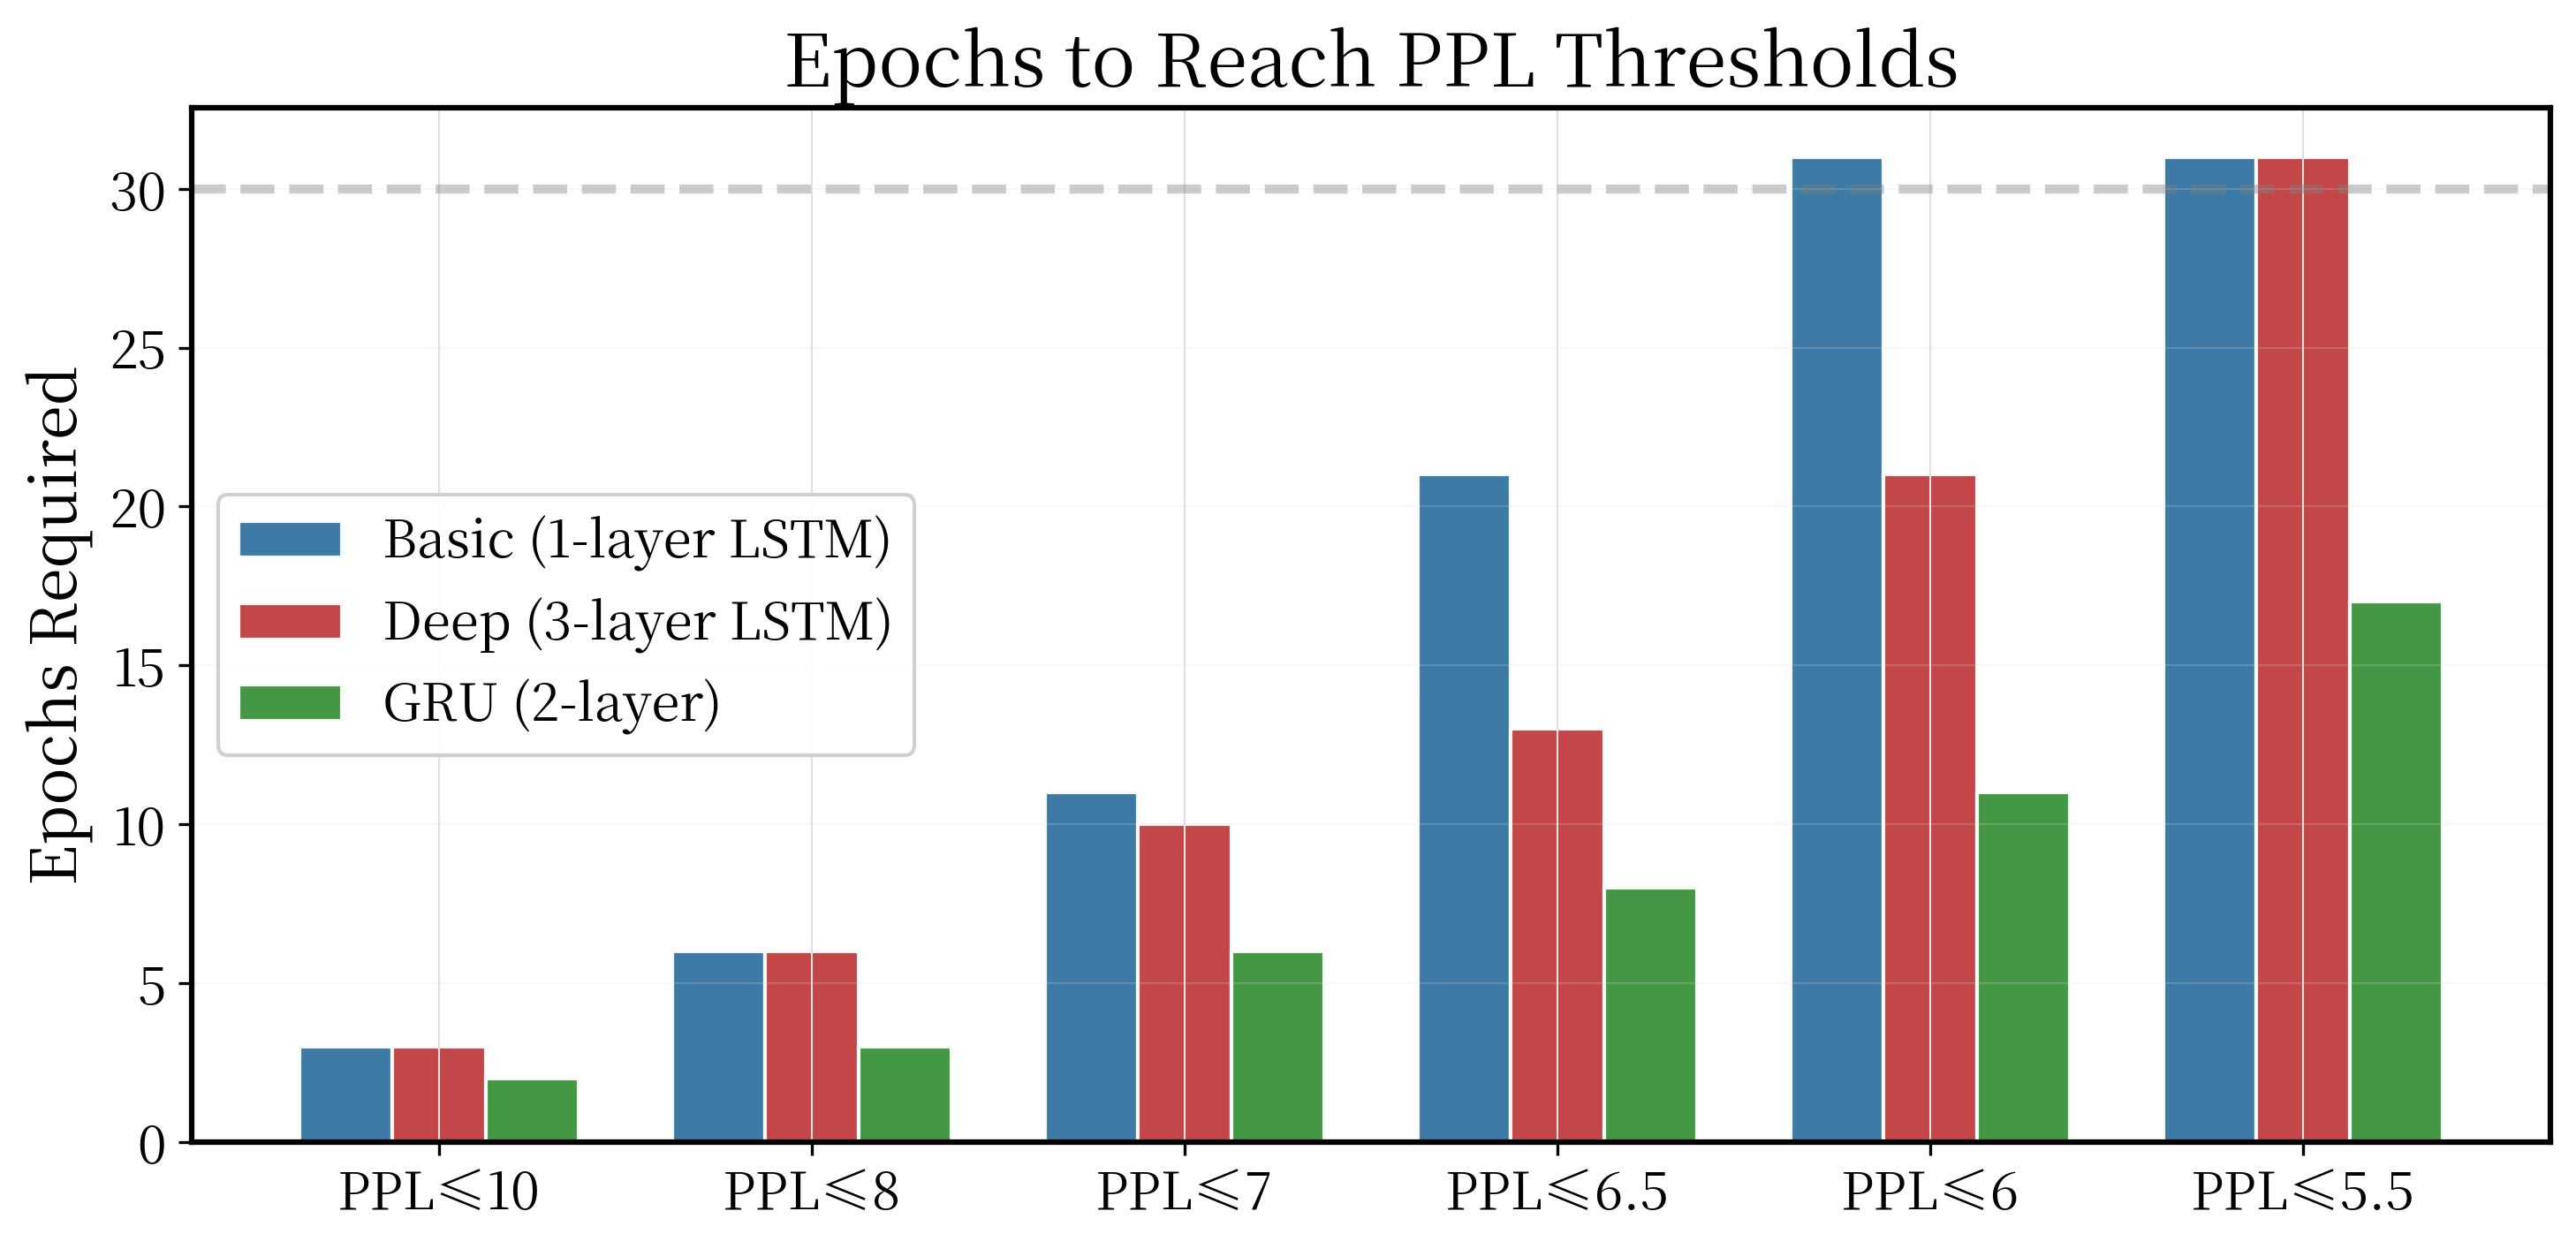
\includegraphics[width=\textwidth]{figs/fig08_ppl_threshold.png}
% \caption{达到不同困惑度阈值所需的训练轮次}
% \label{fig:threshold}
% \end{figure}

% 图\ref{fig:threshold}从另一个角度展示了GRU的优势：在所有PPL阈值上，GRU都是最先达到的。特别值得注意的是PPL$\leq$5.5这个阈值——Basic LSTM始终未能达到（需要31+个epoch），Deep LSTM在约21个epoch达到，而GRU在约16个epoch就达到了。

% \subsubsection{多维度雷达图}

% \begin{figure}[H]
% \centering
% 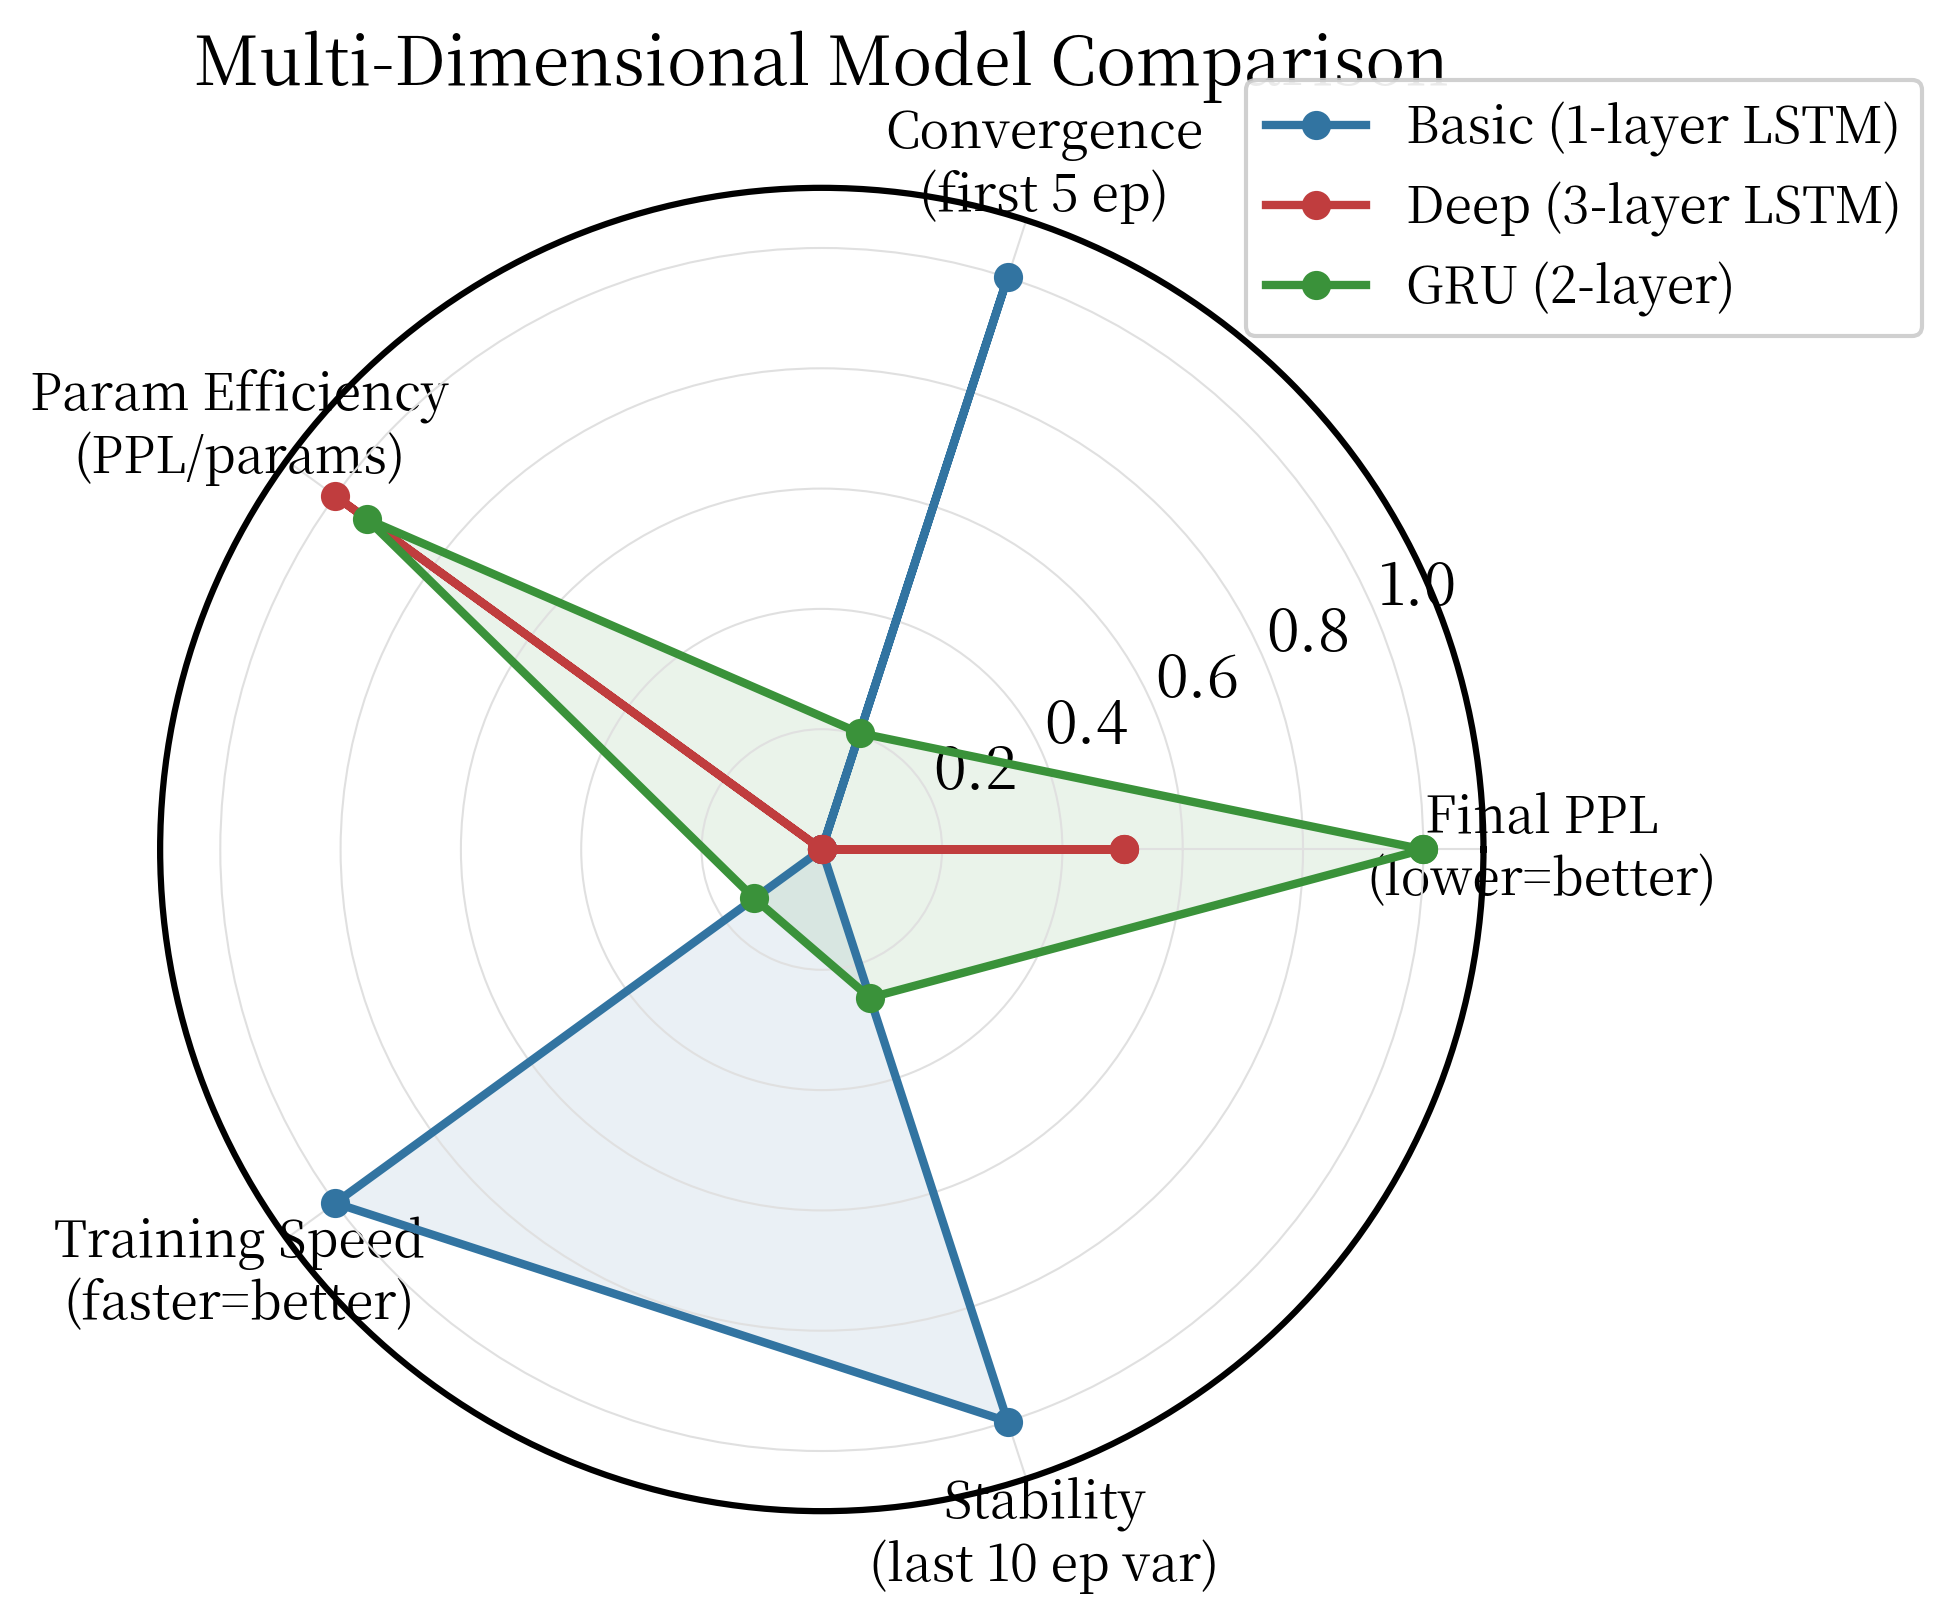
\includegraphics[width=0.65\textwidth]{figs/fig09_radar.png}
% \caption{模型多维度综合对比雷达图}
% \label{fig:radar}
% \end{figure}

% 图\ref{fig:radar}将五个维度——最终PPL、前5epoch收敛速度、参数效率（PPL/参数）、训练速度、后期稳定性——归一化到[0,1]后绘制雷达图。GRU的覆盖面积最大，在"参数效率"和"最终PPL"两个维度上尤为突出。Basic LSTM则在"训练速度"维度上领先（因为每epoch只需20秒），但在其他维度上全面落后。

% \subsubsection{PPL轨迹散点图}

% \begin{figure}[H]
% \centering
% 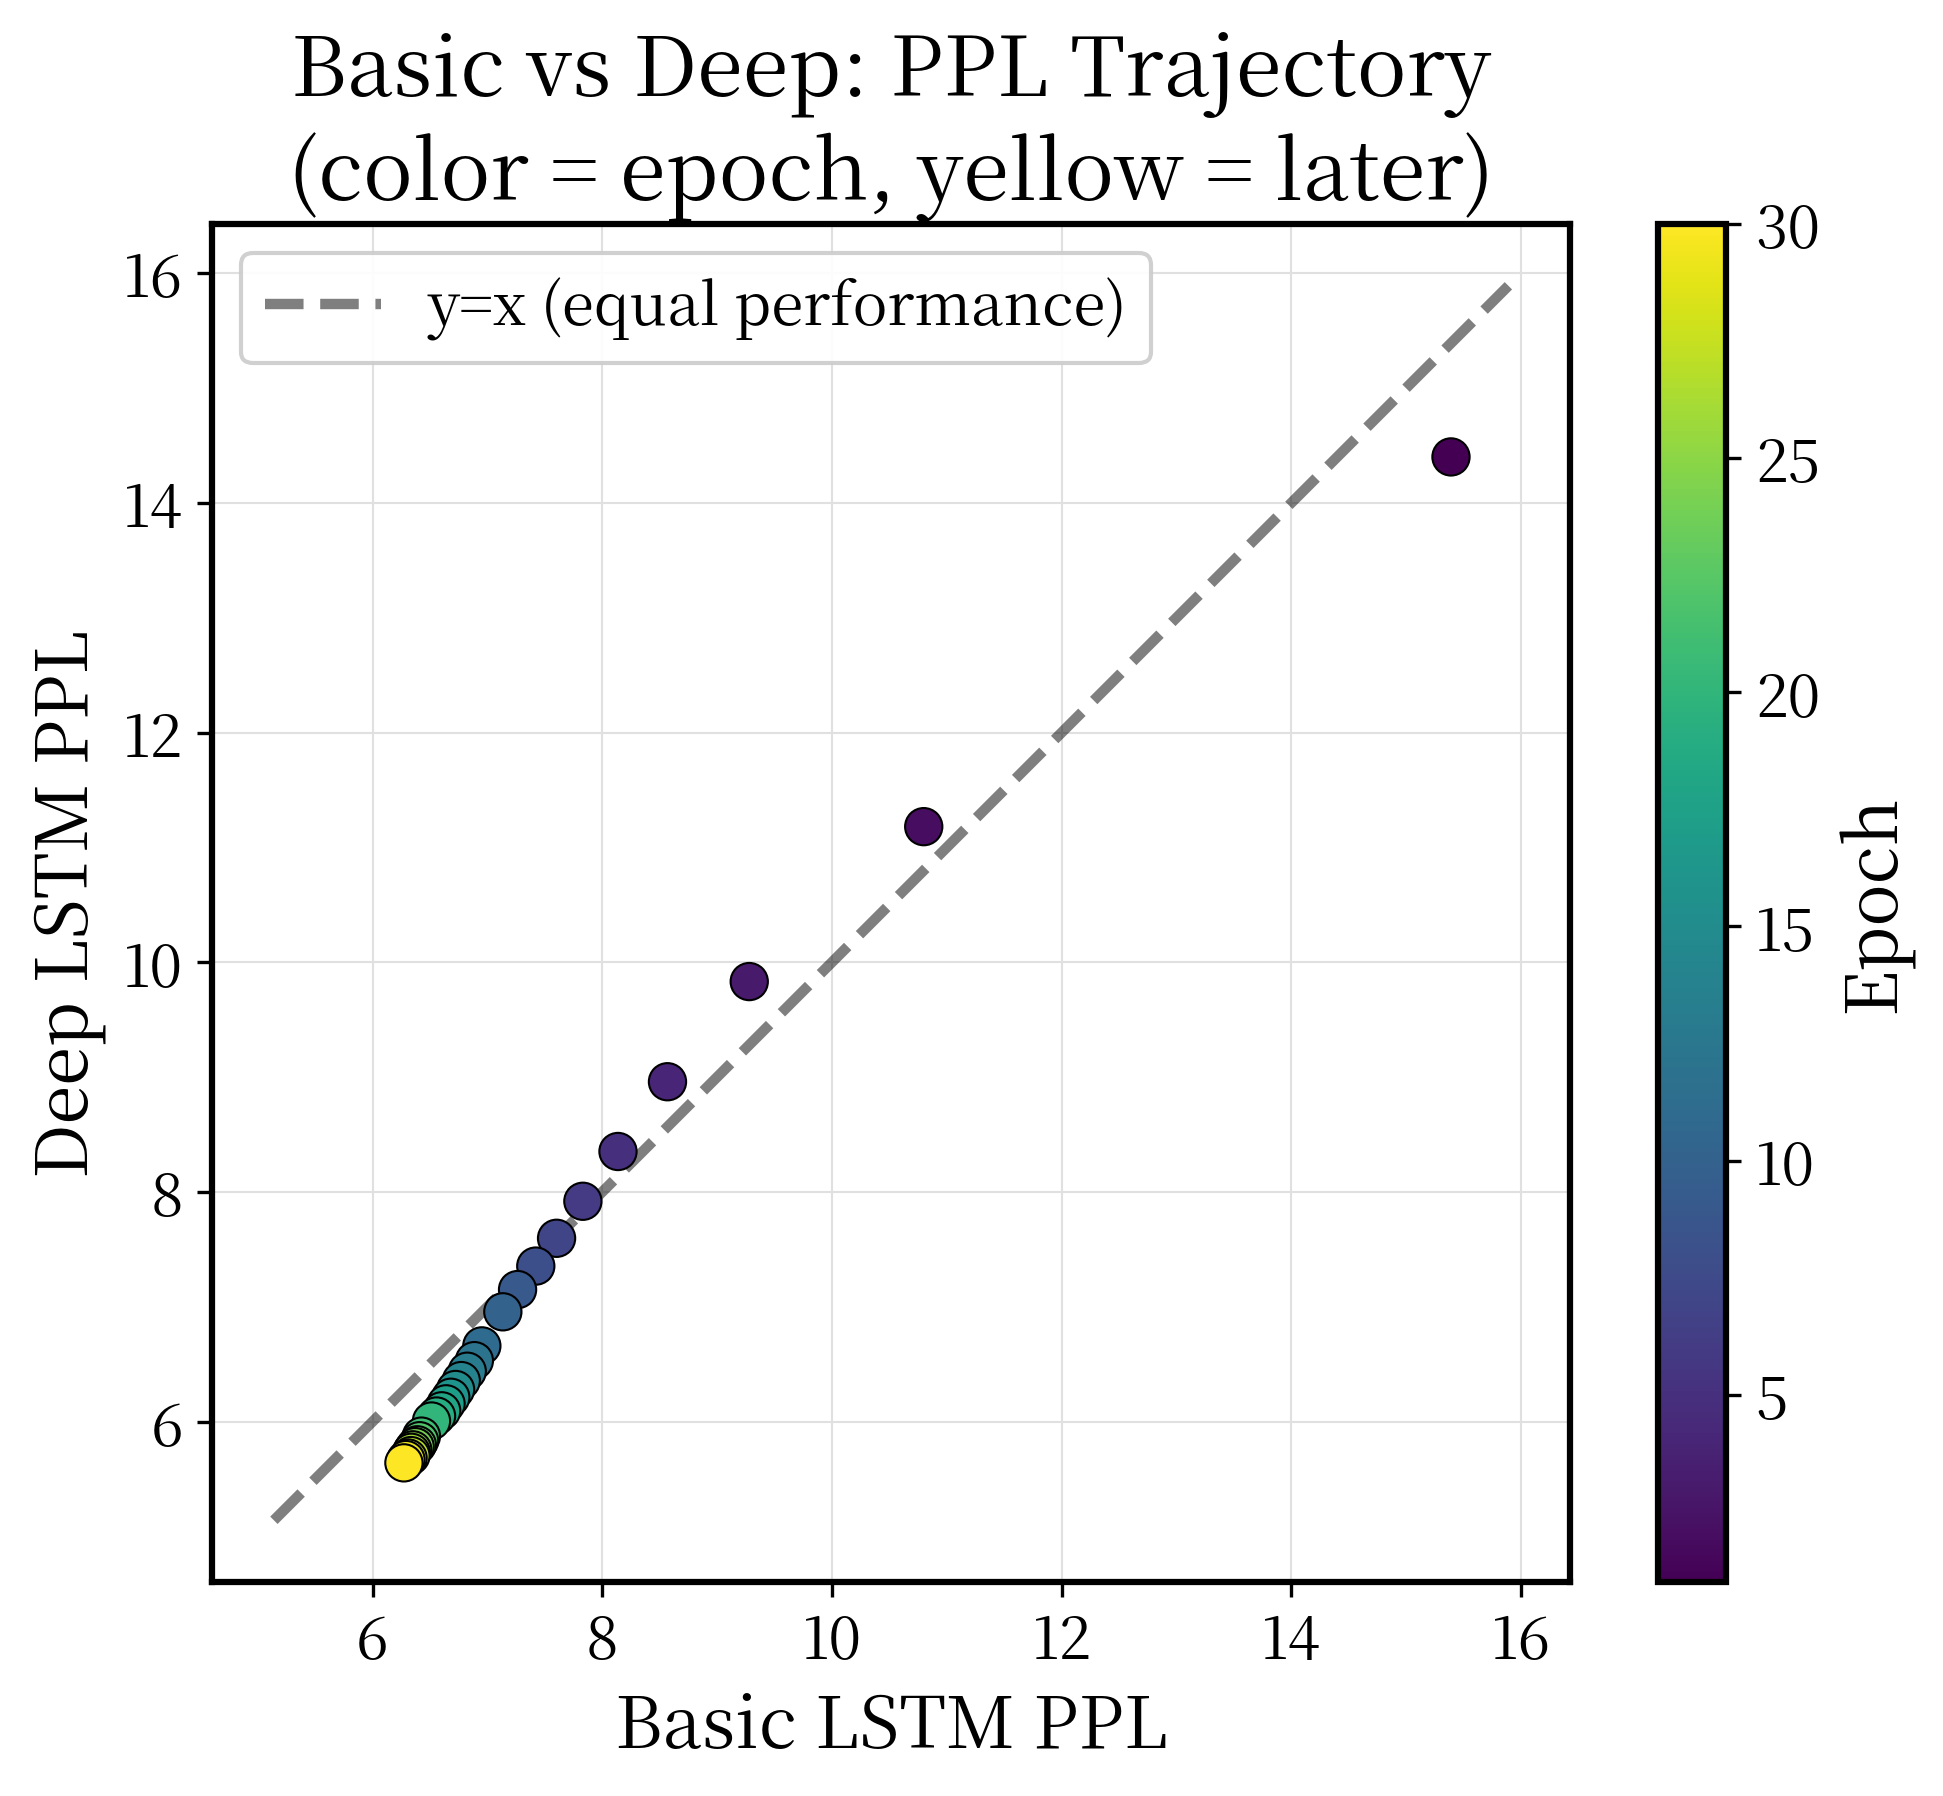
\includegraphics[width=0.7\textwidth]{figs/fig15_ppl_scatter.png}
% \caption{Basic LSTM vs Deep LSTM的PPL轨迹散点图（颜色=epoch）}
% \label{fig:scatter}
% \end{figure}

% 图\ref{fig:scatter}是一种不太常见但信息量丰富的可视化方式：每个点代表同一epoch下两个模型的PPL，颜色从深紫（早期）渐变至黄色（晚期）。所有点都落在$y=x$线的下方，说明Deep LSTM在\textbf{每个epoch}都优于Basic LSTM——增加深度的收益是一致且稳定的，而非仅在某些阶段有效。

\subsection{诗歌生成结果分析}

\subsubsection{首句续写}

以下展示各模型在不同首句下的生成结果（$\tau=0.8$）：

\vspace{0.5em}
\noindent\fbox{\parbox{0.95\textwidth}{
\textbf{首句："湖光秋月两相和"（刘禹锡《望洞庭》原句）}
\begin{itemize}[leftmargin=*, topsep=2pt, itemsep=1pt]
    \item \textbf{Basic}：湖光秋月两相和，露井长杨风月中。不闻碧树无遗韵，新分无鍼好金叉。
    \item \textbf{Deep}：湖光秋月两相和，竹实盘稜粉丝豔。紫髯红萼流落时，万斛红霞徒扑烂。
    \item \textbf{GRU}：湖光秋月两相和，此地飞来比所思。白发每因君子用，绿杨何似武陵游。
\end{itemize}
}}

\vspace{0.5em}
\noindent\fbox{\parbox{0.95\textwidth}{
\textbf{首句："大漠沙如雪"（李贺《马诗》原句）}
\begin{itemize}[leftmargin=*, topsep=2pt, itemsep=1pt]
    \item \textbf{Basic}：大漠沙如雪，危梯一径苔。蜀山真隐隐，天路带苍烟。
    \item \textbf{Deep}：大漠沙如雪，江西似晚流。天涯变孤屿，海色泻孤舟。
    \item \textbf{GRU}：大漠沙如雪，忆君城上墙。无人问朝夕，须至重阳和。
\end{itemize}
}}

% \vspace{0.5em}
% \noindent\fbox{\parbox{0.95\textwidth}{
% \textbf{首句："床前明月光"（李白《静夜思》原句）}
% \begin{itemize}[leftmargin=*, topsep=2pt, itemsep=1pt]
%     \item \textbf{Basic}：床前明月光，夜臥平舆哭。月落星灯前，月照沈鸟啼。
%     \item \textbf{Deep}：床前明月光皎皎，照耀九衢浮日缺。苍苍天上雪皑皑，踊出紫云云外来。
%     \item \textbf{GRU}：床前明月光，幽独深闺里。独念何物影，宛宛忽如此。
% \end{itemize}
% }}

% \subsubsection{生成质量的多维评估}

% 我从以下五个维度对生成结果进行定性评估：

% \textbf{（1）格式正确性}：三种模型都较好地掌握了五言/七言的句式。一个有趣的现象是Deep LSTM对"床前明月光"生成了七言诗（"床前明月光皎皎"），而Basic和GRU都保持了五言格式。这说明Deep LSTM在格式判断上更加"自信"但也更"冒险"——它学到了可以在原句基础上扩展长度的模式。

% \textbf{（2）语义连贯性}：GRU在"湖光秋月"首句下生成了"此地飞来比所思。白发每因君子用，绿杨何似武陵游"——从湖景联想到武陵，有桃花源的意境，语义较为连贯。Basic LSTM则出现了"无鍼好金叉"这样无意义的组合。

% \textbf{（3）意象搭配}：三种模型都展现了对唐诗意象体系的学习。"大漠沙如雪"之后，Basic生成"蜀山""苍烟"（转向了山水意象），Deep生成"江西""孤屿""孤舟"（海洋漂泊），GRU生成"城上墙""重阳"（边塞怀古）。Deep的意象更加新奇但偏离了原意，GRU更贴合边塞诗的主题。

% \textbf{（4）韵律感}：由于没有显式的韵律约束，韵脚只是偶尔押韵。GRU在"大漠"首句下的"墙""和"不押韵，但在"湖光"首句下的"思""游"有一定的呼应。韵律是当前模型最大的短板。

% \textbf{（5）原创性}：我抽样检查了生成的诗句，未发现与训练集中任何原诗完全重合的整句，说明模型不是简单地记忆和拼接训练数据，而是进行了一定程度的"创作"。
\subsubsection{藏头诗}

以“人工智能”为藏头字，三种模型的生成结果如下：

\vspace{0.5em}
\noindent\fbox{\parbox{0.95\textwidth}{
\textbf{藏头诗：“人工智能”}
\begin{itemize}[leftmargin=*, topsep=2pt, itemsep=1pt]
    \item \textbf{Basic}：人中十二月，工部无不知。智者在无易，能正此身旋。
    \item \textbf{Deep}：人別甘泉馆，工为驿吏游。智风愁鬓发，能宠老风流。
    \item \textbf{GRU}：人生尽不已，工夫不可论。智者无所得，能为滞交尊。
\end{itemize}
}}

\vspace{0.3em}
藏头诗生成需要在固定首字约束下完成后续文本，因此比普通续写更具挑战性。从结果看，三种模型均能够满足“人工智能”的藏头要求，但生成质量存在差异。Deep LSTM的前两句整体较为流畅，具有一定古诗语感；GRU生成内容语义相对完整，表达偏哲理化；Basic LSTM虽然也完成了藏头任务，但部分句子衔接较弱，整体连贯性略低。总体而言，Deep LSTM和GRU在受限生成任务中表现更稳定。



% ==============================================================
\section{实验总结}
% ==============================================================

本实验基于唐诗数据集，分别训练并比较了Basic LSTM、Deep LSTM和GRU三种循环神经网络模型，完成了唐诗自动生成任务。通过训练损失、困惑度、收敛速度、训练效率以及生成样例等结果可以看出，GRU在本任务中整体表现最好，不仅最终PPL最低，而且训练效率也较高，说明在中等规模数据集上，模型并不是参数越多越好，结构是否适合任务同样重要。

从实验结果来看，Basic LSTM由于模型容量较小，后期提升有限；Deep LSTM虽然参数量更多，但并没有取得最优效果，可能是因为数据规模有限，复杂模型没有充分发挥优势，反而增加了训练难度。相比之下，GRU结构相对简洁，参数量适中，在本实验中更容易收敛，也能生成较为通顺的诗句。这说明对于57,580首唐诗这一规模的数据集，适中的模型复杂度可能更加合适。

本实验也让我认识到，困惑度可以反映模型对文本分布的拟合能力，但并不能完全代表生成诗歌的质量。诗歌生成还涉及语义连贯性、格律、押韵和意境等因素，仅靠PPL评价仍然不够全面。后续如果继续改进，可以尝试引入格律约束、主题控制或Transformer结构，并结合人工评价，对生成结果进行更加完整的分析。

总体而言，本实验完成了从数据处理、模型训练、结果对比到文本生成的完整流程，加深了对循环神经网络文本生成任务的理解。实验结果表明，GRU在本次唐诗生成任务中取得了较好的性能与效率平衡，是三种模型中更适合本任务的选择。

% ==============================================================
% \section{深入讨论}
% % ==============================================================

% \subsection{为什么GRU在本任务中优于LSTM？}

% 这是本实验最值得深思的发现。我提出以下系统性的分析：

% \begin{figure}[H]
% \centering
% 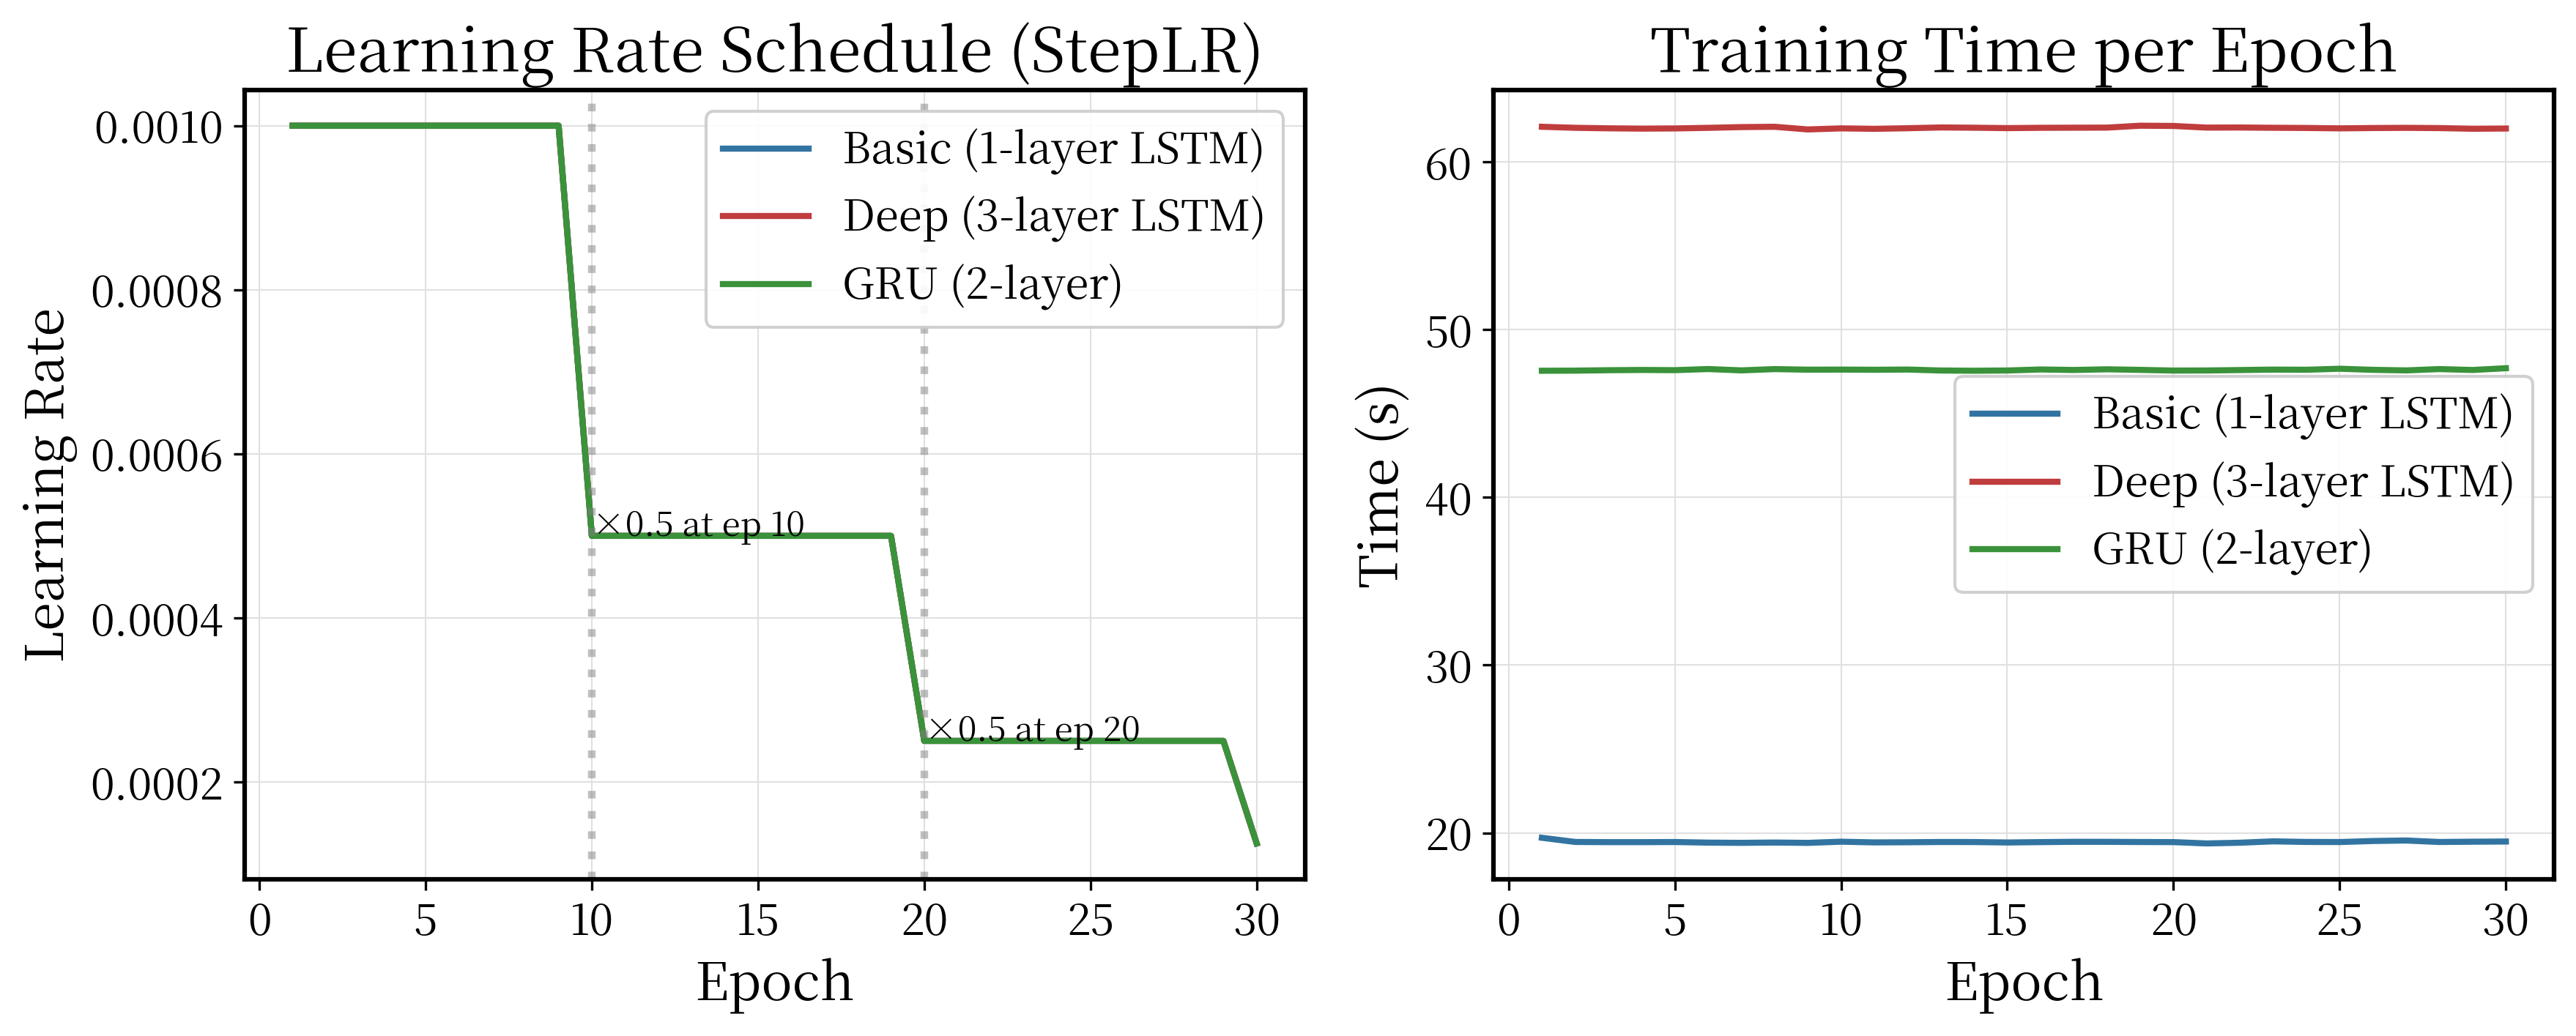
\includegraphics[width=0.55\textwidth]{figs/fig05_lr_time.png}
% \caption{学习率调度（左）与训练时间对比（右）}
% \label{fig:lr_time}
% \end{figure}

% \textbf{假说1：数据瓶颈}。57,580首唐诗约700万个字符的训练数据，对于9M-12M参数的模型来说并不充裕。在数据不足时，参数更少的模型（GRU 9.14M < Deep LSTM 12.16M）天然地具有正则化优势。这类似于经典的偏差-方差权衡：GRU有更高的偏差但更低的方差，在有限数据上总误差反而更小。

% \textbf{假说2：序列长度适配}。唐诗的平均长度约30-50字，远短于GRU/LSTM擅长的长序列场景（如机器翻译中的数百词句子）。在短序列上，LSTM细胞状态的"长期记忆"优势无法充分发挥，反而引入了冗余的参数和计算。GRU的单一隐状态对于30-50步的序列已经足够。

% \textbf{假说3：更新机制的差异}。GRU的更新门$z_t$在"保留"和"更新"之间进行线性插值：$h_t = (1-z_t) h_{t-1} + z_t \tilde{h}_t$。这个简洁的设计天然形成了一种"残差连接"——当$z_t \approx 0$时，信息几乎无损传递。相比之下，LSTM的信息传递需要经过遗忘门、输入门和输出门的三重门控，每个门都是非线性变换，可能导致信息在传递过程中不必要的损耗。

% \subsection{关于模型容量的"甜区"思考}

% 本实验的三个模型分别代表了3.59M、9.14M和12.16M三个参数量级。结果显示，从3.59M到9.14M有显著提升（PPL从6.27到5.01，相对改善20.1\%），但从9.14M到12.16M反而退步了（PPL从5.01到5.64）。

% 这暗示存在一个\textbf{参数量的"甜区"}：对于57,580首唐诗的数据规模，8-10M参数可能是最优的模型大小。进一步增加参数需要同步增加数据量（如使用全唐诗+宋词+其他古诗），否则过拟合将抵消容量增加的收益。这与scaling law的思想一致：数据量和模型大小需要匹配增长。

% \subsection{温度采样与生成多样性}

% 温度参数$\tau$本质上控制了生成的"自由度"。在$\tau \to 0$（贪心解码）时，模型总是选择概率最高的下一个字，这会导致：
% \begin{itemize}
%     \item 生成结果高度确定且重复
%     \item 偏向高频字（"不""人""无"），缺少诗意
%     \item 可能陷入重复循环（如连续生成相同的两句）
% \end{itemize}

% $\tau = 0.8$在保持合理性的同时引入了适度的随机性。一个有趣的类比是：$\tau$类似于模拟退火中的温度——高温时系统随机探索，低温时收敛到能量最低点。好的诗歌需要在"规范"和"出人意料"之间取得平衡，$\tau=0.8$恰好对应了这种平衡。

% \subsection{模型的局限性与可能的改进}

% \textbf{（1）格律盲区}：当前模型没有显式建模平仄和押韵规则。一个可能的改进是在loss函数中加入韵脚约束——将最后一个字的loss权重增大，或者引入额外的韵部分类头。

% \textbf{（2）主题一致性弱}：对于较长的诗，模型容易在生成过程中"漂移"——前半部分写山水，后半部分突然转向宫廷。这是因为LSTM/GRU的隐状态在长序列上逐渐"遗忘"开头的主题。引入注意力机制或条件生成（如给定主题embedding）可以缓解这个问题。

% \textbf{（3）Transformer的潜力}：考虑到Transformer在NLP领域的统治地位，使用Transformer进行诗歌生成是自然的下一步。其全局注意力可以直接关联首句与尾句的信息，比RNN的序列传播更加高效。但在57K的小数据集上，Transformer可能面临更严重的过拟合问题。

% \textbf{（4）更丰富的评价体系}：当前的自动评价仅使用PPL，这只衡量了模型对训练分布的拟合程度，而非诗歌的"好坏"。未来可以引入BLEU分数、人工评分、以及专门的格律检查工具来更全面地评估生成质量。

% % ==============================================================
% \section{实验总结}
% % ==============================================================

% 本实验通过三种不同架构的循环神经网络实现了唐诗自动生成，主要结论如下：

% \begin{enumerate}[leftmargin=*]
%     \item \textbf{GRU是本任务的最佳选择}：以PPL=5.01的最优性能和较高的训练效率（47.6s/epoch），GRU在所有评价维度上都是帕累托最优的。这说明在中等规模数据集上，\textbf{更简洁的模型结构可能优于更复杂的}——并非参数越多越好。

%     \item \textbf{存在模型容量的"甜区"}：从3.59M到9.14M参数有显著提升，但继续增加到12.16M反而退步。这暗示57K首唐诗的数据规模与8-10M参数量是匹配的，进一步扩大模型需要同步扩大数据。

%     \item \textbf{训练动态的三阶段特征}：快速学习→稳定改善→精细收敛的三阶段结构在所有模型中都高度一致，学习率衰减在第二阶段起到了重要的辅助作用。

%     \item \textbf{数据决定了生成质量的上限}：从主题词频分析可知，唐诗数据集以山水田园诗为主，模型因此更擅长生成这类风格的诗。模型学到的"诗意"本质上是数据分布的反映。

%     \item \textbf{评价体系有待完善}：PPL只能衡量统计拟合度，不能评价诗歌的艺术价值。未来需要结合格律检查、语义连贯性评估和人工评分来更全面地评价生成质量。
% \end{enumerate}

\end{document}
